\section{Introduction to general relativity}

    At the heart of Albert Einstein's general theory of relativity lies a profound shift in our understanding of gravity and space-time. In this section, we'll delve into the qualitative aspects of general relativity and draw comparisons with its predecessor, special relativity.\\

    One of the central tenets of general relativity is the idea that massive objects, like planets and stars, bend the fabric of space-time around them. This bending, often depicted as a curved surface, is what we perceive as gravity. Imagine placing a heavy ball on a stretched rubber sheet. The sheet curves around the ball, and smaller objects nearby naturally roll toward it. Similarly, massive objects create curves in space-time, influencing the motion of other objects in their vicinity.

    This insight was a monumental departure from the classical concept of gravity as a force of attraction between masses. Rather than envisioning a force acting at a distance, general relativity describes gravity as a consequence of the geometry of space-time itself.\\

    Special relativity, introduced by Einstein in 1905, focuses on the relationship between space and time, particularly in situations involving relative motion. It famously established the constancy of the speed of light, which led to phenomena like time dilation and length contraction. Special relativity was designed to address situations where velocities approach the speed of light and encompassed the realm of "inertial frames" – frames that move at a constant velocity relative to one another.

    General relativity extends this framework to non-inertial frames – those undergoing acceleration or influenced by gravitational fields. It unifies gravity with the fabric of space-time, encompassing all motion, including accelerated motion, within its purview. While special relativity deals with flat space-time and relative motion, general relativity introduces the dynamic curvature of space-time itself as a response to mass and energy.\\

    One of the remarkable consequences of general relativity is its application to the cosmological scale. The curvature of space-time influences the trajectory of light, causing gravitational lensing – the bending of light around massive objects. This effect was confirmed during the 1919 solar eclipse observations, where stars near the Sun appeared slightly shifted due to the bending of their light around the Sun's gravitational field.\\

    General relativity also provides the foundation for understanding black holes, where the gravitational curvature becomes so intense that not even light can escape – leading to the concept of an event horizon. These celestial phenomena have since become crucial tools for studying the universe's most extreme environments and for testing the boundaries of our understanding of physics.

    In summary, general relativity profoundly transformed our understanding of gravity by revealing it as the result of the curvature of space-time caused by mass and energy. This departure from the classical Newtonian view revolutionized our comprehension of the cosmos, offering a unified description of gravity and motion on all scales.

    While special relativity opened the door to the intertwining of space and time and addressed relative motion in inertial frames, general relativity extended this framework to include accelerated motion and the gravitational influence of massive objects. Together, these theories form the foundation of modern physics, guiding our exploration of the universe's inner workings and shaping our technological advancements.

    \subsection{The incompatibility between the Newtonian gravity with the special relativity}

        The Newton's universal law of gravity was one of the biggest hits in the history of physics, this is because he could explain almost all the gravitational phenomena in the planet (or any other) and in the solar system, with this theory Edmund Halley could also predict the trajectory of a far asteroid, the well known Halley's asteroid. The Newton's theory failed with one special planet in the solar system, Mercury, no one could explain the retrograde movement of this planet using this theory, it was Albert Einstein with his theory of general relativity who could solve this problem and generalize to high gravitational fields and also discovered that his theory of special relativity is incompatible with the Newton's theory.\\

        Lets show that. The SR (special relativity from now on) has preferred observers \footnote{here we must clarify that a preferred observer is not a coordinate card, an observer is related to world trajectories, therefore the observers are related more to a geometrical objetcs.} this are known as \textit{inertial observers} when we associate then with a set of four coordinates ,$(t,x,y,z)$, this becomes an inertial reference frame. The different inertial frames are all related by Lorentz transformations, with this we can enunciate the \textit{principle of special relativity}.

        \begin{myPrinciple}
            \textbf{Principle of special relavitiy:} The laws of physics must take the same form in every inertial frame.
        \end{myPrinciple}

        This principle talks about the mathematical forms of the laws of physics this means that no matter how you transform the reference frame, the coordinate system, the mathematical form of the laws must be the same, there is no physical interest in a mathematical formulation fro a physical law which has a different form for every inertial frame.\\

        Lets analyze the Newton's laws to see like this the compatibility between this and the SR

        \begin{equation}\label{eq:NewtonLawGrav}
            \nabla^2 \phi = 4\pi G\rho
        \end{equation}

        where $\phi$ is the gravitational potential, $\rho$ is the mass density, and $G$ is the gravitational or Cavendish's constant. Due to the Lorentz transformations the spatial and temporal coordinates mix each other it is obvious that this equations won't be longer a Poisson equation under a Lorentz transformation, this implies that \textit{the Newton laws are incompatible with the principle of special relativity}.  So now lets analyze the behaviour of the solutions of the equation \ref{eq:NewtonLawGrav}, these have the form,

        \begin{equation}
            \phi(t,\Vec{x}) = -G\int \frac{\rho(t,\Vec{x}')}{|\Vec{x}-\Vec{x}'|}d^3x',
        \end{equation}

        solutions of this form also violate the principle of SR, because solutions of this from have instantaneous reactions which also violate the principles because \textit{two simultaneous events (spatially separated) in an inertial reference frame, wont be simultaneous en all the other reference frames.}\\

        It is worth to wonder when are compatible the SR with the Newtonian gravity, we will prove that this compatibility is given under low velocities, when we talk about low velocities we must say respect to what, from now on in the context of the relativity theory usually is respect to the speed of light $C$, so when $v \ll C$ like in the solar system. All the planets in or solar system travel, in a relatively good approximation, in circular trajectories so we can use the Newtons's law and the gravitation law to relate the potential with the speed, the gravitational potential is

        \begin{equation}
            \phi = - \frac{M G}{|\Vec{r}|}
        \end{equation}

        where $M$ is the sun's mass, and $\Vec{r}$ is the positions vector from the sun to the planet, if the movement is perfectly circular there is a centripetal acceleration, thus

        \begin{equation}
            \frac{GM}{|\Vec{r}|^2} = \frac{v^2}{|\Vec{r}|} \rightarrow \frac{v^2}{C^2} = \frac{|\phi|}{C^2}.
        \end{equation}

        Here we can see the direct relation there is between the gravitational potential with the relativistic effects in gravitational fields, intense gravitational fields imply relativistic effects, this also implies, yeh again, \textit{the Newton theory is incompatible with relativity.} When $|\phi| / C^2 \ll 1$ we have that the Newton's law are compatible. There is a certain dimensionless constant that tell us if an object is enough to produce relativistc effects, this is called the compactness $c$ defined by:

        \begin{equation}
            c = \frac{GM}{C^2r}.
        \end{equation}

        This constant for the sun has a values of the order of $\approx 10^{-6}$ and for a Neutron star of $\approx 0.5$, thus in the vicinity of a Neutron star the relativistic effects will be really important in contrast with our sun.

    \subsection{Weak equivalence principle}

        In the Newtonian theory there is a difference between two concepts, the \textit{inertial mass} and the \textit{gravitational mass} , $m_I,m_g$ respectively, the distinctions between these two is really important, because in the common language, they're the same, but we will see that the fact they're numerically the same implies a principle and they are not the same concepts, physically imply two different things.

        \begin{itemize}
            \item The inertial mass is related with the second law of Newton, this mass is an inertia factor wich tell us how hard would be to move and object and appears mathematically as

            \begin{equation}
                \Vec{F} = m_I \Vec{a}.
            \end{equation}

            \item The gravitational mass is a factors which tell us how an object interacts with a gravitational field it is the analogous to charge in the electromagnetism and appears mathematically as

            \begin{equation}
                \Vec{F} = m_g \Vec{g}.
            \end{equation}
        \end{itemize}

        To see how are they related, lets consider a particle falling freely in a gravitational field, thus

        \begin{equation}
            \Vec{a} = \frac{\Vec{F}}{m_I} = \frac{m_g}{m_I}\Vec{g}.
        \end{equation}

        It was Galileo, with his so famous experiments in the Piza tower, who postulate \textit{the relation between the gravitational and inertial mass $m_g/m_I$ are the same for all the materials}. Without any loss of generality, we're saying that in magnitude the gravitational mass and the inertial mass are equal. Later Eötvös proved experimentally that

        \begin{equation}\label{eq:EotvosRel}
            \frac{m_g}{m_I} - 1 \approx \mathcal{O}(10^{-12}).
        \end{equation}

        This separates the gravity respect to all the other three forces, because all the other forces interact with matter depending on their compositions but this not, the main objective nowadays is to try to violate the relations \ref{eq:EotvosRel} and we can say that \textit{the equality between $m_I$ and $m_g$ for all the bodies is a form of the weak equivalence principle}.\\

        The relation \ref{eq:EotvosRel}, this principle, in fact has a really heavy implication mathematically, because we start from a movement equation like,

        \begin{equation}
            m_I\Ddot{\Vec{x}} = m_g \Vec{g}[\Vec{x}(t),t],
        \end{equation}

        but using \ref{eq:EotvosRel} we then get

        \begin{equation}
            \Ddot{\Vec{x}} =  \Vec{g}[\Vec{x}(t),t].
        \end{equation}

        Solutions of this equations are determined uniquely byt the initial position and speed of the particle. This implies that \textbf{two different particle with the same position and speed will have the same trajectories.} Without this relation this wont be any longer true, there is the strenght and beauty of this principle. Lets now formulate this principle in this other, but physically equal, form:

        \begin{myPrinciple}
            \textbf{Weak equivalence principle:} The trajectory of a test body falling freely depends only on its initial position and speed and it is independent of is chemical composition.
        \end{myPrinciple}

        We must remember that this is enunciate to test bodies, this kind of test bodies have got auto-gravitational effects negligible respect to the field of the sources and this is not extended, it is almost a particle respect to the field size, this to avoid effects like torques.  Lets analyze the mechanical behavior of a reference frame that fulfill the transformations of Galileo's group.

        \begin{align}
            t' = t ,\\
            \Vec{X}' = \Vec{X} - \Vec{Y}(t),
        \end{align}

        $\Vec{Y}(t)$ is related with the origin of the new reference frame. And we will set $\Ddot{\Vec{Y}}(t) = \Vec{a}$ so the acceleration of the new reference frame is given by the Galileo's relativity theory by

        \begin{equation}\label{eq: xdobleprim}
            \Ddot{\Vec{X}}' = \Vec{g} - \Vec{a} = \Vec{g}'.
        \end{equation}

        Here we can see the acceleration of the new reference frame can be interpreted as a measure of the gravity acceleration from this reference frame, lets analyze some special cases of the equation \ref{eq: xdobleprim}.

        \begin{enumerate}
            \item $\Vec{g} = 0$ which implies that $\Vec{g}' = - \Vec{a}$ we can see that \textit{the uniform acceleration is indistinguishable from an uniform gravitational acceleration.}

            \item $\Vec{g} = cte \;\; \& \;\; \Vec{a} = \Vec{g}$. For this kind of situations we can then find an inertial reference frame associated to the free fall, in this reference frame the gravitational effects are zero. This is equivalent to be next to a falling object like a paratrooper. 
        \end{enumerate}

        If we haven't got uniformity, then we will see that \textit{each coordinate chard of the inertial reference frame can be such that this is associated to a geometrical manifold, such manifolds will allow us to define neighborhoods which are locally Minkowskian.}

    \subsection{Experimental evidence for a general relativity theory}

        Many physics students feel attraction to the theory of general relativity and gravitation because the mathematical structure behind this theory which by its own is really abstract but with this theory it takes a beautiful physical interpretation but many people forget how this theory was born. \\

        Is the experimentation, the experiences we live everyday what allow physicist do physics, because of that there are some experiments which cannot be explained with the special relativity theory of which are the first steps in the search of a general theory of relativity, here we're going to check some of those experiments and analyze their physical information.

        \subsubsection{Eötvös experiment}

            The Hungarian Baron Loránd Eötvös was a mathematician, engineer and physicist who made an amazing experiment to test the equivalence principle, here we're going to analyze his experiment. Lets suppose a pair of objects to which a force is applied 

            \begin{align}
                \Vec{F}^{(1)} = m_I^{(1)}\Vec{a}^{(1)} = m_g^{(1)}\Vec{g},\\
                \Vec{F}^{(1)} = m_I^{(2)}\Vec{a}^{(2)} = m_g^{(2)}\Vec{g}.
            \end{align}

            He, in his experiment, postulate that the acceleration of the two objects aren't the same

            \begin{equation}
                \Vec{a}^{(2)} = \frac{m_g^{(2)}}{m_I^{(2)}}\Vec{g} \neq \frac{m_g^{(1)}}{m_I^{(1)}}\Vec{g} = \Vec{a}^{(1)}.
            \end{equation}

            We're going to have on count the gravitational force

            \begin{equation}
                \Vec{F}_g = -G M_OM_G \frac{\Vec{r}}{r^3},
            \end{equation}

            and the centrifugal force due to the relative rotational motion between the two forces with angular frequency $\Vec{\omega}$, see figure \ref{fig:CircularTrjectory}.

            \begin{figure}[h]
                \centering
                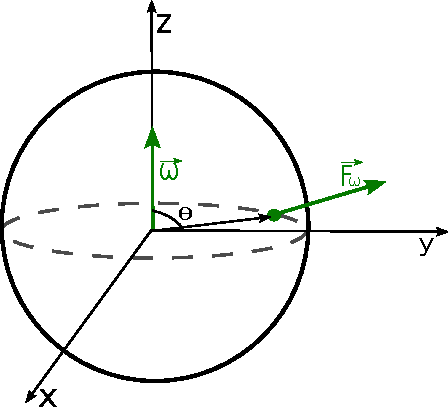
\includegraphics[width = 0.5\textwidth]{Chapter 3/Figures/CircularTrajectory.pdf}
                \caption{Graphical representation of the relative movement between the two test bodies.}
                \label{fig:CircularTrjectory}
            \end{figure}

            \begin{align}\label{eq:Raxis}
                \Vec{F}_{\omega} = m_I\omega^2 \Vec{r}_{axis},\\
                \Vec{r}_{axis} = \Vec{r}- \frac{(\Vec{\omega}\cdot\Vec{r})}{\omega^2}\Vec{\omega},
            \end{align}

            \begin{equation}
                \Vec{F}_{\omega} = m_I \left[\Vec{\omega}\times(\Vec{\omega}\times\Vec{r})\right].
            \end{equation}

            Then the forces balance is

            \begin{equation*}
                \Vec{F}^{(i)} = \Vec{F}_g^{(i)} + \Vec{F}_{\omega}^{(i)}.
            \end{equation*}

            And lets define a parameter $\alpha$ which relates the strength relation between the gravitational and centrifugal force as

            \begin{equation}
                \alpha = \frac{\left| \Vec{F}^{(1)} \times \Vec{F}^{(2)} \right|}{|\Vec{F}^{(1)}||\Vec{F}^{(2)}|},
            \end{equation}

            if $\alpha = 0$ we'll have that the forces are parallel. In magnitude in the earth the gravitational force is stronger than the centrifugal because 

            \begin{equation*}
                \frac{G M_O}{|\Vec{r}|} / \frac{1}{\omega^2 |\Vec{r}|^2}\approx 300.
            \end{equation*}

            Lets calculate the parameter $\alpha$ so, first we're going to calculate the numerator

            \begin{align*}
                \Vec{F}^{(1)}\times\Vec{F^{(2)}} = \left( -GM_Om_g^{(1)}\frac{\Vec{r}}{r^3} + m_I^{(1)} \left[\Vec{\omega}\times (\Vec{\omega}\times \Vec{r})\right] \right) \times \left( -GM_Om_g^{(2)}\frac{\Vec{r}}{r^3} + m_I^{(2)} \left[\Vec{\omega}\times (\Vec{\omega}\times \Vec{r})\right] \right)\\
                = - \left(\frac{GM_Om_g^{(1)}m_I^{(2)}}{r^3}\right)(\Vec{r}\times\Vec{\omega})\times(\Vec{\omega}\times\Vec{r}) - \left(\frac{GM_Om_g^{(2)}m_I^{(1)}}{r^3}\right)\left[\Vec{\omega}\times(\Vec{\omega}\times\Vec{r})\right]\times\Vec{r}\\
                = -\frac{GM_O\omega^2}{r^3}\left\{m_g^{(1)}m_I^{(2)}\Vec{r}\times \left[\Vec{r} - \frac{(\Vec{\omega}\cdot\Vec{r})\Vec{\omega}}{\omega^2}\right] - m_g^{(2)}m_I^{(1)}\left[\Vec{r} - \frac{(\Vec{\omega}\cdot\Vec{r})\Vec{\omega}}{\omega^2}\right] \times \Vec{r} \right\}\\
                = -\frac{GM_O}{r^3}(\Vec{r}\times\Vec{\omega})(\Vec{\omega}\cdot\Vec{r})[m_g^{(1)}m_I^{(2)} - m_g^{(2)}m_I^{(1)}],
            \end{align*}

            \begin{equation}
                \left|\Vec{F}^{(1)}\times \Vec{F}^{(2)}\right| = \frac{GM_O}{r^3}|\Vec{r}\times\Vec{\omega}|(\Vec{\omega}\cdot\Vec{r})[m_g^{(1)}m_I^{(2)} - m_g^{(2)}m_I^{(1)}].
            \end{equation}

            Now, for the denominator we must calculate each norm, because both have the same form we'll do for one and only change their respective indices

            \begin{align*}
                |\Vec{F}^{(i)}| = \left\{\frac{(GM_Om_g^{(i)})^2}{r^4} + (m_I^{(i)}\omega^2)^2 \left[\Vec{r} - \frac{(\Vec{\omega}\cdot\Vec{r})\Vec{\omega}}{\omega^2}\right]\cdot\left[\Vec{r} - \frac{(\Vec{\omega}\cdot\Vec{r})\Vec{\omega}}{\omega^2}\right] -2GM_Om_g^{(i)}m_I^{(i)}\frac{\omega^2}{r^3}\Vec{r}\cdot\left[\Vec{r} - \frac{(\Vec{\omega}\cdot\Vec{r})\Vec{\omega}}{\omega^2}\right]\right\}^{1/2}\\
                =\left\{ \frac{(GM_Om_g^{(i)})^2}{r^4} + (m_I^{(i)}\omega^2)^2\left[r^2 - \frac{2 (\Vec{\omega}\cdot\Vec{r})^2}{\omega^2} + \frac{(\Vec{\omega}\cdot\Vec{r})^2}{\omega^2}\right] - 2GM_Om_g^{(i)}m_I^{(i)}\frac{\omega^2}{r^3}\left[r^2 - \frac{(\Vec{\omega}\cdot\Vec{r})^2}{\omega^2}\right] \right\}^{1/2}\\
                =  \frac{GM_Om_g^{(i)}}{r^2}\left\{1 + \left[\frac{m_I^{(i)}\omega^2}{GM_Om_g^{(i)}}\right]\left[r^2 - \frac{(\Vec{\omega}\cdot\Vec{r})^2}{\omega^2}\right]\left[\frac{m_i^{(i)}r^2\omega^2}{GM_Om_g^{(i)}} - \frac{2}{r}\right]\right\}^{1/2}.
            \end{align*}

            Taking a first order aproximation, or what is the same, saying the biggest contribution to the norm of each force is due to the gravitational interaction we then have:

            \begin{equation}
                |\Vec{F}^{(i)}| \approx \frac{GM_Om_g^{(i)}}{r^2},
            \end{equation}

            then the parameter $\alpha$ becomes

            \begin{equation}
                \alpha \approx \left[\frac{m_I^{(1)}}{m_g^{(1)}} - \frac{m_I^{(2)}}{m_g^{(2)}} \right] \frac{|\Vec{r}\times\Vec{\omega}|(\Vec{\omega}\cdot\Vec{r})}{GM_O},
            \end{equation}

            \begin{equation}\label{eq:alphaparameter}
                \alpha \approx \left[\frac{m_I^{(1)}}{m_g^{(1)}} - \frac{m_I^{(2)}}{m_g^{(2)}} \right] \frac{cos\theta sin\theta}{300}.
            \end{equation}

            With the result of the equation \ref{eq:alphaparameter} we can see that this experiment can not be done for some who is in the equator nor the poles because $\theta = 0 \;\&\; \theta = \pi/2$ respectively, fortunately Eötvös was in Hungary a country beyond the equator and he found that $\alpha$ was zero in a part for $10^9$, this means it is zero until the ninth significant number, from there on there are errors, and mathematically from \ref{eq:alphaparameter} we can see that if it is zero this means by the elementary theorem of algebra that 

            \begin{equation}
                \frac{m_I^{(1)}}{m_g^{(1)}} = \frac{m_I^{(2)}}{m_g^{(2)}}.
            \end{equation}

        \subsubsection{Tidal forces}

            \begin{figure}[h]
                \centering
                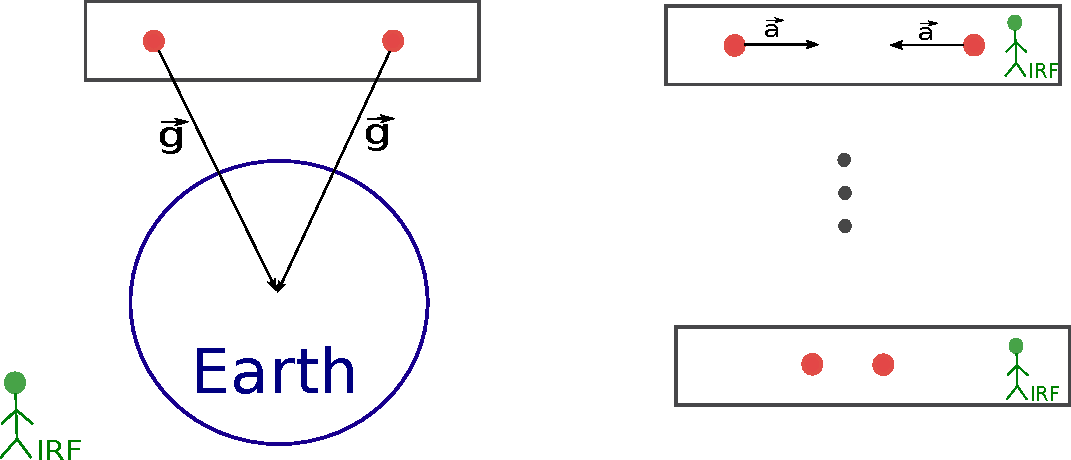
\includegraphics[width = 0.7\textwidth]{Chapter 3/Figures/TidalForces.pdf}
                \caption{In the left there are two particles which are in a free fall to the earth an the inertial reference frame (IRF) is to the side of the earth, he observes a diagonal trajectory of the bodies. In the right we set the IRF inside the box with the two bodies, and he observes that there is a strange force which makes the bodies get together.}
                \label{fig:TidalForces}
            \end{figure}

            In the figure \ref{fig:TidalForces} we can see an scheme of the effect of the tidal forces on two particles inside a box. This box is in a free fall to the earth, a observer with an inertial reference frame next to the earth will observe a kind of diagonal trajectory for both particle to the center of the earth but if we place our inertial reference frame inside the box we will see that both particles will join together why? In the Newtonian mechanics we would say that there is a fictitious force \footnote{Newton never used the term fictitious force, that term was introduce by the Mach's formalism for the mechanics.} that makes the objects attract each other but in fact, there is no imaginary force, there is a non homogeneous gravitational field, so \textit{the tidal forces are an effect of the non homogeneity of the gravitational field, these are physical and important forces.}

        \subsubsection{Light deflection and gravitational red shift}

            \begin{figure}[h]
                \centering
                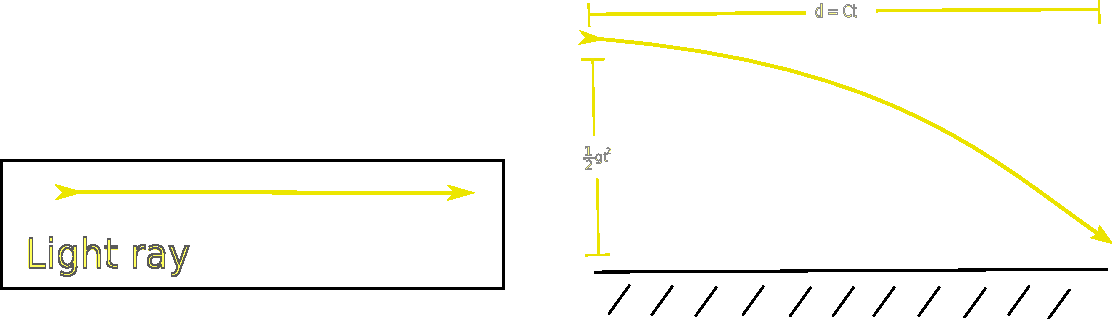
\includegraphics[width = 0.9\textwidth]{Chapter 3/Figures/LightDeflection.pdf}
                \caption{In the left there is a light ray seeing from an inertial reference frame inside the box, and in the right there is the same ray but seeing from the earth.}
                \label{fig:light deflection}
            \end{figure}

            In the figure \ref{fig:CircularTrjectory} we can see that even the light is affected by the gravity, in the Newtonian theory this was something impossible to imagine!, we need then a theory to describe this effect.\\

            There are some other effects of the gravity on the light, like the color shift, this is a gravitational Doppler effect, so, lets suppose two observers Alice (A) and Bob (B), Alice is in a free fall at a distance $h$ from Bob and sends a light pulse, then Bob gets it and in the moment he gets it Alice sends another beam what is the relation between the Alice and bob interval times?. To solve this we will suppose the gravity is uniform and we will set a reference frame such that $\Vec{g} = \Vec{a}$ so for Alice 

            \begin{align}
                Z_A = h + \frac{1}{2}gt^2\\
                Z_B = \frac{1}{2}gt^2.
            \end{align}

            Alice sends the first signal at a time $t_1$ then the position of the beam $Z$ is

            \begin{align}
                Z = Z_A(t_1) - C(t-t_1) = h + \frac{1}{2}gt_1^2 - C(t-t_1),
            \end{align}

            it arrives to Bob at $t = T_1$ then

            \begin{equation}\label{eq:desa1}
                h + \frac{1}{2}gt_1^2 - C(T_1 - t_1) = \frac{1}{2}gT_1^2.
            \end{equation}

            Alice sends the second signal at $t = t_1 + \triangle \tau_A$ then

            \begin{equation}
                Z = Z_A(t_1 + \triangle \tau_A) - C(t - t_1 - \triangle\tau_A).
            \end{equation}

            And it lands on Bob at $t = T_1 + \triangle \tau_B$ thus

            \begin{equation}\label{eq:desa2}
                h + \frac{1}{2}g(t_1 + \triangle\tau_A)^2 - C(T_1 + \triangle \tau_B - t_1 - \triangle\tau_A) = \frac{1}{2}g(T_1 + \triangle\tau_B)^2
            \end{equation}

            Lest expand \ref{eq:desa2} then

            \begin{align}
                h + \frac{1}{2}g(t_1+\triangle\tau_A)^2 - C(T_1 + \triangle\tau_B - t_1 - \triangle\tau_A) = \frac{1}{2}g(T_1 + \triangle\tau_B)^2,\\
                h + \frac{1}{2}g(t_1^2 + 2t_1\triangle\tau_A + \triangle\tau_A^2) - C(T_1 + \triangle\tau_B - t_1 - \triangle\tau_A) = \frac{1}{2}g(T_1^2 + 2T_1\triangle\tau_B + \triangle\tau_B^2).
            \end{align}

            Using the equation \ref{eq:desa1} in the right hand side of the last equation and simplifying the $h$ and $\frac{1}{2}gt_1^2$ then we have

            \begin{align*}
                gt_1\triangle\tau_A + \frac{1}{2}g\triangle\tau_A^2 - C(\triangle\tau_B - \triangle\tau_A) = gT_1\triangle\tau_B + \frac{1}{2}g\triangle\tau_B^2,\\
                \triangle\tau_A(gt_1+C) + \frac{1}{2}g\triangle\tau_a^2 = \triangle\tau_B(gT_1 + C) + \frac{1}{2}g\triangle\tau_B^2.
            \end{align*}

            Dividing all by $C$ and remembering that in Earth $g\triangle\tau_i \ll C$ then we have

            \begin{equation}
                \triangle \tau_A \left(1 + \frac{gt_1}{C}\right) = \triangle\tau_B\left(1 + \frac{gT_1}{C}\right)
            \end{equation}

            \begin{equation}
                \triangle \tau_B = \left(1 + \frac{gt_1}{C}\right)\left(1 + \frac{gT_1}{C}\right)^{-1}\triangle\tau_A,
            \end{equation}

            now using the geometric series $\frac{1}{1+x} = 1 - x + x^2 - x^3 + ...$ to first order because, in the Earth $gt_i \leq C$ thus

            \begin{equation}
                \triangle\tau_B \approx \left[1 + \frac{gt_1}{C} - \frac{gT_1}{C} - g^2\frac{t_1T_1}{C^2}\right]\triangle\tau_A \approx \left[1 - \frac{g}{C}(T_1-t_1)\right]\triangle\tau_A.
            \end{equation}

            The times seems to run slower in $B$ than in $A$ we can conclude then that \textit{the time runs slower where the gravitational field is stronger.} Here we can also see two things, the first one is that the compactness appears again because

            \begin{equation}
                \triangle\tau_B \approx \left[1 - \frac{gh}{C^2}\right]\triangle\tau_A = \left[1 +\frac{\phi_B - \phi_A}{C^2})\right]\triangle\tau_A,
            \end{equation}

            then we see the compactness appears and tells us how fast will run the time of an observer. The other thing we can see is a blue shift because using the relation between time and frequency $\triangle\tau_i = \frac{\lambda_i}{C}$ we then have

            \begin{equation}
                \lambda_B \approx \left(1 - \frac{gh}{C^2}\right)\lambda_A
            \end{equation}

            and because the second term in the parenthesis is positive the wavelength of $Bob$ will be each time shorter, show there will be a blue shift, or what is the same a Doppler effect when the ambulance (Alice with her laser) comes closer to Bob.

    \subsection{Einstein's equivalence principle and the space-time}

        Einstein introduced the space-time structure to his theory, this to make a coupled theory of space and time, in the Newtonian theory the space is absolute and the time is absolute but not together, this was the Einstein's contribution to physics, neither time nor space are absolute separately but joint they are, such a structure has a special geometry, called a pseudo-Reinmannian geometry, this because in these geometríes there are negative and positive or even null vector modulus , their physical interpretation will be discused later. A space-time diagram is a representation of the physical events, for example for the blue shift problem the diagram is represented in the figure \ref{fig:Spacetimediagram}.

        \begin{figure}[h]
            \centering
            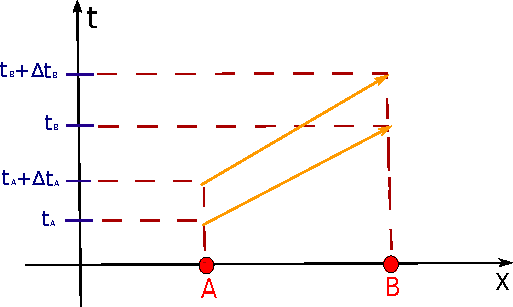
\includegraphics[width = 0.7\textwidth]{Chapter 3/Figures/Spacetimediagram.pdf}
            \caption{Space-time diagram representation for the Doppler effect analized before.}
            \label{fig:Spacetimediagram}
        \end{figure}

        Lets study this, in a Minkowskian structure we have got the following relation

        \begin{equation}
            C^3d\tau^2 = C^2dt^2 - dx^2 - dy^2 - dz^2,
        \end{equation}

        but lets see what happens if we modify it a bit like this

        \begin{equation}\label{eq:nonMinkowski}
            C^2d\tau^2 = \left(1 + \frac{2\phi}{C^2}\right)C^2dt^2 - \left(1 - \frac{2\phi}{C^2}\right)(dx^2+dy^2+dz^2),
        \end{equation}

        as we can see for Alice and Bob there are no physical displacement, only temporal, so their proper times are, using the equation \ref{eq:nonMinkowski} are

        \begin{align}
            \triangle\tau_A^2 = \left(1 + \frac{2\phi_A}{C^2}\right)\triangle t^2,\\
            \triangle\tau_B^2 = \left(1 + \frac{2\phi_B}{C^2}\right)\triangle t^2.
        \end{align}

        Now, taking the square root of both equations and using Taylor expansion to first order we then have

        \begin{align}
            \triangle\tau_A \approx \left(1 + \frac{\phi_A}{C^2}\right)\triangle t,\\
            \triangle\tau_B \approx \left(1 + \frac{\phi_B}{C^2}\right)\triangle t.
        \end{align}

        It is easy to see that the relation between their proper times is 

        \begin{equation}
            \triangle\tau_B \approx \left(1 + \frac{\phi_B}{C^2}\right) \left(1 + \frac{\phi_A}{C^2}\right)^{-1}
        \end{equation}

        Using now the geometrical series because in the earth the compactness is really low $\phi/C^2 \ll 1$ finally we then have

        \begin{equation}
            \triangle\tau_B\approx \left(1 + \frac{\phi_B - \phi_A}{C^2}\right)\triangle\tau_A.
        \end{equation}

        This is a really strong result because changing the plane geometric structure of the Minkowskian space-time we will return the result we had obtain before with the light blue shift, this is a straight proof that we need a more geometrical an general theory of the relativity.

\section{First steps on general relativity}

    From now on me will move to a more physical territory using all the abstract tools developed by the mathematicians, first we're going to learn how to craw, then to walk and at the end how to run, because the general relativity is in fact a theory of \textit{the electrodynamics of bodies in movement} the heart of a movement, from a physical point of view, is the notion of position and even more important, the notion of distance, this in mathematics, in a topological space can be defined using a topoly on the topological space, here in the same way we're going to define a metric on the manifold, what we will call a metric tensor.

    \subsection{Metric tensor}

        Lets see how to make the notion of distance over $M$, for example, lets look at $\mathbb{R}^3$. Let $\Vec{X}(t)$ a curve on $\mathbb{R}^3$ and an open interval $a < t < b$ so the arc length $L$ is given by

        \begin{equation}
            L = \int_a^b ds = \int_a^b \left[\frac{d\Vec{X}}{dt}\cdot \frac{d\Vec{X}}{dt}\right],
        \end{equation}

        where $\Vec{X}$ is the tangent vector to the curve, we see here rises the notion of inner product of these tangent vectors does it mean that always an inner product give us a notion of distance? The fast answer is yes, but the long answer is no, the notion of inner product is more related to the notion of a topology of the vector space, in our case of the tangent space to a point $p$ on the manifold $M$.\\

        The notion of distance is a kind of combinations between the notion of topology or inner product with the physical structure of the problem, there are many maps or inner products that satisfies the axioms of a topology or the inner product is the physical meaning what rises the notion of distance, therefore to find such a distance lets define the metric tensor $\mathbb{G}$

        \begin{equation}
            \mathbb{G}\;:\; T_p(M)\times T_p(M) \rightarrow \mathbb{R},
        \end{equation}

        and in our notation the application of the metric tensor $\mathbb{G}$ to two vectors is

        \begin{equation}
            \mathbb{G}(\Vec{A},\Vec{B}) = \Vec{A}\cdot\Vec{B}.
        \end{equation}

        \begin{myDef}
            A metric tensor in $p\in M$ is a tensor $\mathbb{G}$ of type $\binom{0}{2}$, known also as bilinear form, such that satisfies the following properties:

            \begin{enumerate}
                \item $\mathbb{G}(\Vec{X},\Vec{Y}) = \mathbb{G}(\Vec{Y},\Vec{X}) \;\forall \; \Vec{X},\Vec{Y}\; \in T_p(M).$

                \item $\mathbb{G}(\Vec{X},\Vec{Y}) = 0 \;\forall \;\Vec{Y}\;\in T_p \; \Leftrightarrow \; \Vec{X} = \Vec{0}$ this means the metric tensor is not degenerated.
            \end{enumerate}
        \end{myDef}

        In differential geometry we're always interested in a metric such that it is Riemannian this means \textit{the metric has a signature mostly positive}, this means the metric tensor is positive-defined. In general relativity we're interested in Lorentizan metrics, they are those whose signature has the form $-\;+\;+\;...$ here the metric is not necessarily positive-defined.

        \begin{myDef}
            A Riemannian manifold es a pair $(M,\mathbb{G})$ where $M$ is a differentiable manifold and $\mathbb{G}$ is the metric tensor field, which can be Riemannian or not.\\

            In general relativity such a pair is known as \textit{space-time}.
        \end{myDef}

        In this way we can calculate a length curve $L$ as

        \begin{equation}
            L = \int_a^b \left[\mathbb
            {G}(\Vec{X},\Vec{X})\right]^{1/2}_{\lambda(t)},
        \end{equation}

        and given a coordinate chart we can write the metric tensor as

        \begin{equation}
            \mathbb{G} = g_{\alpha\beta}dx^{\alpha}\otimes dx^{\beta}.
        \end{equation}

        \begin{myDef}
            The metric $\mathbb{G}$ is not degenerated, thus this must be invertible. Te inverse metric is a symmetric tensor field of type $\binom{2}{0}$ denoted by $\mathbb{G}^{-1}$ such that

            \begin{equation}
                g^{ac}g_{cb} = \delta^a_{\;b}.
            \end{equation}
        \end{myDef}

        \begin{myDef}
            The Lorentzian signature is defined such that for any point $p$ in the manifold we can choose an orthonormal basis $\{\mathbf{e}_{\alpha}\}$ such that

            \begin{equation}
                \mathbb{G}(\mathbf{e}_{\alpha},\mathbf{e}_{\beta}) = g_{\alpha\beta} \equiv Diagonal[-1,1,1,1,1,...].
            \end{equation}
        \end{myDef}

        This basis is not unique and we must set a relation between basis

        \begin{align*}
            \mathbf{e}_{\Bar{\alpha}} = \Lambda^{\beta}_{\Bar{\alpha}}\mathbf{e}_{\beta}\rightarrow g_{\Bar{\alpha}\Bar{\beta}} = \mathbb{G}(\mathbf{e}_{\Bar{\alpha}},\mathbf{e}_{\Bar{\beta}}) = \mathbb{G}\left(\Lambda^{\mu}_{\;\Bar{\alpha}}\mathbf{e}_{\mu}, \Lambda^{\nu}_{\;\Bar{\beta}}\mathbf{e}_{\nu}\right)\\
            = \Lambda^{\mu}_{\;\Bar{\alpha}}\Lambda^{\nu}_{\;\Bar{\beta}}\mathbb{G}(\mathbf{e}_{\mu},\mathbf{e}_{\nu}) = \Lambda^{\mu}_{\;\Bar{\alpha}}\Lambda^{\nu}_{\;\Bar{\beta}} g_{\mu\nu}.
        \end{align*}

        All the basis are related by Lorentz transformations.

    \subsection{Proper time and an introduction to paths
    }

        Due to the nature of the space-time manifold $(\mathbb{R}^4,\mathbb{G})$ the vectors in this space have a particular behavior.

        \begin{myDef}
            On a Lorentzian manifold $(M,\mathbb{G})$ a non zero vector $\Vec{X}\;\in\;T_p(M)$ is

            \begin{itemize}
                \item A time-like vector $\mathbb{G}\left(\Vec{X},\Vec{X}\right) < 0$.

                \item A null or light-like vector $\mathbb{G}\left(\Vec{X},\Vec{X}\right)=0$.

                \item A space-like vector $\mathbb{G}\left(\Vec{X},\Vec{X}\right)>0$.
            \end{itemize}
        \end{myDef}

        \begin{figure}[h]
            \centering
            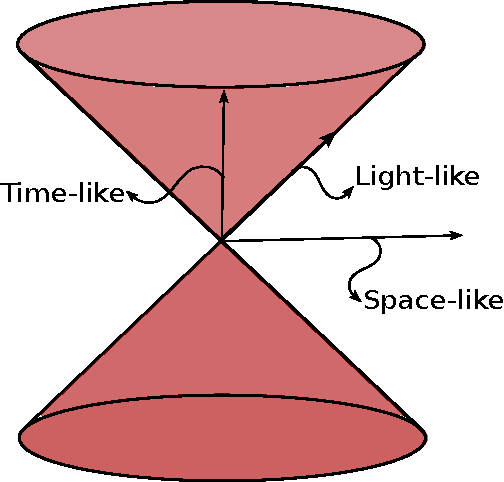
\includegraphics[width = 0.5\textwidth]{Chapter 3/Figures/ConoDeLuz.pdf}
            \caption{The light cone for the space-time structure, in the $x$-axis there is $\mathbb{R}^3$ and in the $y$ axis there is the coordinate time $t$, a space-like vector is a vector which lives outwards the cone, a light-like lives on the border of the cone  and a time-like lives inside the cone.}
            \label{fig:conoLuz}
        \end{figure}

        In the figure \ref{fig:conoLuz} there is a graphical representations of these three kinds of vectors, if we adopt a mostly positive signature, and from the postulates of the special relativity we can see the vectors with physical meaning are the time and light like vectors, because we can reach and not even get over the light speed so everything will be inside the cone and the objects that travel at the speed of light will be on the cone border, a space-link thus wont have any physical meaning.\\

        We will see we can associate an observer with a time-like vector, therefore we'll focus on the properties of these vector, moreover on the characteristics of their tangent space $T_p(M)$, first we must see that if $\{\mathbf{e}_{\mu}\}$ is basis of orthonormal vectors in $p$, then the metric tensor has components

        \begin{equation}
            \mathbb{G}\left(\mathbf{e}_{\alpha},\mathbf{e}_{\mu}\right) = \eta_{\alpha\beta}
        \end{equation}

        such that $T_p(M)$ has exactly the same structure that the Minkowski space-time.\\

        The time-like trajectory in a Lorentizan manifold $\left(M,\mathbb{G}\right)$ is given by an integral curve such that $\Vec{X}$ is always time-like or in a more formal way $\mathbb{G}(\Vec{X},\Vec{X}) < 0$ see figure \ref{fig:TimeCurve}.

        \begin{figure}
            \centering
            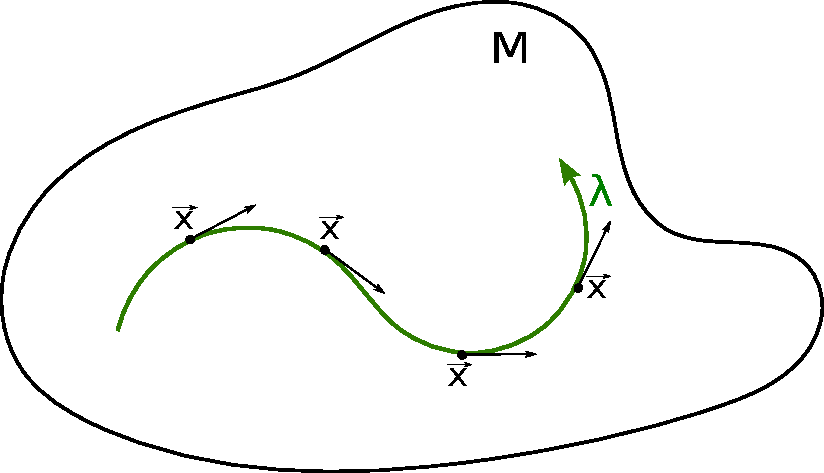
\includegraphics[width = 0.5\textwidth]{Chapter 3/Figures/TimeCurve.pdf}
            \caption{Graphical representation of an integral time-like curve on a manifold $M$.}
            \label{fig:TimeCurve}
        \end{figure}

        Lets see the behavir of this curve. Let $\lambda(v)$ a smooth time-like curve such that $\lambda(0) = p$ and we can find an expression for a tangent vector $\Vec{X}^a$, which is time-like, therefore we can define a proper time

        \begin{equation}
            \frac{d\tau}{dv} = - \sqrt{- \left(g_{ab}\Vec{x}^a\Vec{x}^b\right)|_{\lambda(v)}}\;\;\&\;\; \tau(0) = 0.
        \end{equation}

        We must remember $ds^2 = d\Vec{X}\cdot d\Vec{X} = g_{\alpha\beta}dx^{\alpha}dx^{\beta}$ this is given a coordinate basis in a coordinate chart $\phi = \{x^0,x^1,x^2,x^3\}\;\in\;\mathbb{R}^4$ thus

        \begin{equation}
            \frac{dx^2}{dv^2} = g_{\alpha\beta}\frac{dx^{\alpha}}{dv}\frac{dx^{\beta}}{dv},
        \end{equation}

        using a Minkowski space-time we have

        \begin{equation}
            d\tau^2 = -g_{\mu\nu}dx^{\mu}dx^{\nu} = -ds^2,
        \end{equation}

        this allows us to see that $\Vec{X} = X^{\alpha}\frac{d}{dx^{\alpha}}$ therefore $X^{\alpha} = \frac{dx^{\alpha}}{dv}$ we can then integrate and find an expression for the proper time

        \begin{equation}\label{eq:Tau}
            \tau = \int_0^{v_q}\left[-\left(g_{\mu\nu}\frac{dx^{\mu}}{dv}\frac{dx^{\nu}}{dv}\right)\right]_{\lambda(v)}^{1/2}du.
        \end{equation}

        We will see later that the time-like vectors can be parameterized from a proper time like \ref{eq:Tau}, for the null-like ones we gotta chose an special curve, this is because the equation \ref{eq:Tau} ins related to geodesics. We're going to suppose $v = \tau$, the parameter is the proper time, then developing the equation \ref{eq:Tau}

        \begin{equation*}
            \tau = \int_0^{\tau}\left[-\left(-g_{\mu\nu}\frac{dx^{\mu}}{d\tau}\frac{dx^{\nu}}{d\tau}\right)\right]^{1/2}d\tau,
        \end{equation*}

        \begin{equation*}
            \tau = \int_0^{\tau}\left[-U^{\mu}U_{\mu}\right]^{1/2}d\tau.
        \end{equation*}

        For the expression \ref{eq:Tau} become the proper time, we gotta impose that the tangent quadri-vector has norm $-1$ for any coordinate chart.\\

        In the study of mechanics there is an important question, what is the path a test particle will follow in certain conditions? And why,from an infinity family of trajectories, did the particle choose its trajectory? To answer this a mathematical theory was developed, what we in physics known as the variational principles, let $M$ a manifold and $\lambda(\tau)$ a time-like integral curve on $M$ and $\lambda(\tau')$ alternative integral curves, see figure \ref{fig:Variational}, thus the proper time is given by

        \begin{figure}[h]
            \centering
            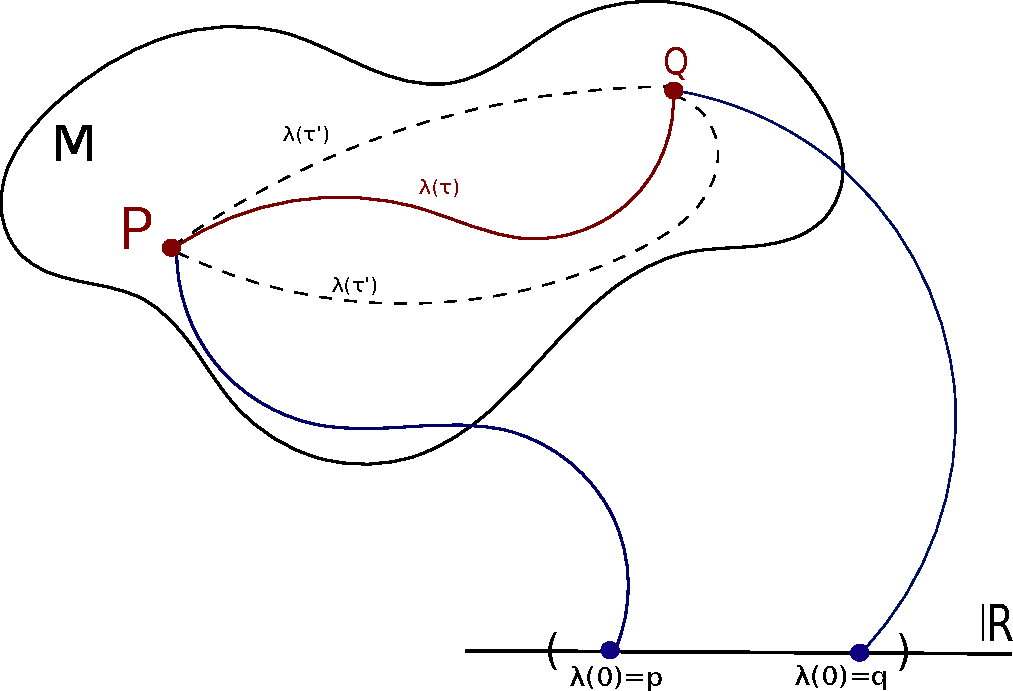
\includegraphics[width=0.5\textwidth]{Chapter 3/Figures/Variational.pdf}
            \caption{The real time-like trajectory a particle will follow is $\lambda(\tau)$ and the other two will be little different trajectories but with initial an final points fixed.}
            \label{fig:Variational}
        \end{figure}

        \begin{equation}\label{eq:variational2}
            \tau\left[\lambda(v)\right] = \int_0^1 G\left(x\left(\lambda(v)\right), \Dot{x}\left(\lambda\left(v\right)\right)\right)du,
        \end{equation}

        \begin{equation}\label{eq:Ghalf}
            G = \left[-g_{\mu\nu}\left(x\left(\lambda(v)\right)\right)\Dot{x}^{\mu}\left(\lambda(v)\right)\Dot{x}^{\nu}\left(\lambda(v)\right)\right]^{1/2},
        \end{equation}

        Using the equations \ref{eq:variational2} and \ref{eq:Ghalf} we want to formulate the following problem, how must be the magnitude of the metric $G$ such that the proper time is stationary this means, it is minimum, or maximum or a seat value. Lets find time-like curve $\lambda(v)$ to extreme the integral \ref{eq:variational2}.\\

        Let us denote the correct chart as $x(\lambda)$ and the incorrect one as 

        \begin{equation}
            X(\lambda) = x(\lambda) + \eta(\lambda),
        \end{equation}

        where $\eta(\lambda$ is  the difference between the real and the wrong path, and because the initial and end point are fixed, thus

        \begin{equation}
            \eta\left(\lambda(0) \right) = \eta\left(\lambda(1) \right) = 0.
        \end{equation}

        The integral $\tau\left[\lambda\right]$ taken along the wrong curve $X(\lambda)$ must be larger than that along the right curve $x(\lambda)$, no matter how close the former is to the latter. To express this requirement, we will introduce a parameter $\alpha$ and redefine $X(\lambda)$ to be

        \begin{equation}\label{eq:alphaeta}
            X(\lambda) = x(\lambda) + \alpha\eta(\lambda),
        \end{equation}

        The integral S taken along the curve $X(\lambda)$ now depends on the parameter $\alpha$, so lets all it call it $\tau(\alpha)$. The right curve $x(\lambda)$ is obtained from \ref{eq:alphaeta} by setting $\alpha=0$. Thus the requirement that $\tau$ is minimum for the right curve $x(\lambda)$ implies that $\tau(\alpha)$ is stationary at $\alpha=0$. With this result, we have converted our problem to the traditional problem from elementary calculus of making sure that an ordinary function [namely $\tau(\alpha)$] has a minimum at $\alpha$ specified point $\alpha=0$. To ensure this, we must just check that the derivative $\frac{d\tau}{d\alpha}$ is zero when $\alpha=0$.

        The integral $\tau(\alpha)$ is

        \begin{equation}\label{eq:IntTovar}
            \tau(\alpha) = \int_{0}^{1}G\left(x(\lambda),\Dot{x}(\lambda),\lambda \right)dv = \int_{0}^{1}G\left(x + \alpha\eta , \Dot{x} + \alpha\Dot{\eta}\right)dv.
        \end{equation}

        To differentiate \ref{eq:IntTovar} with respect to a, we note that a appears in the integrand $G$, so we need to evaluate a $\frac{\partial G}{\partial\alpha}$. Since $\alpha$ appears in two of the arguments of $G$, this gives two terms, namely (using the chain rule)

        \begin{equation}
            \frac{\partial G\left(x + \alpha\eta , \Dot{x} + \alpha \Dot{\eta},\lambda \right)}{\partial \alpha} = \eta\frac{\partial G}{\partial x} + \Dot{\eta}\frac{\partial G}{\partial \Dot{x}},
        \end{equation}

        and for $\frac{d\tau}{d\alpha}$ which has to be zero

        \begin{equation}\label{eq:dtaudalph}
            \frac{d\tau}{d\alpha} = \int_0^1\frac{\partial G}{\partial \alpha}dv = \int_0^1\left(\eta\frac{\partial G}{\partial x^{\mu}} + \Dot{\eta}\frac{\partial G}{\partial \Dot{x}^{\mu}} \right)dv=0.
        \end{equation}

        We need to rewrite the second term on the right using integration by parts'

        \begin{equation}
            \int_0^1\Dot{\eta}(\lambda)\frac{\partial G}{\partial \Dot{x}^{\mu} } = \left[\eta(\lambda) \frac{\partial G}{\partial \Dot{x}^{\mu}} \right]_0^1 - \int_0^1\eta(\lambda)\frac{d}{d\lambda}\left(\frac{G}{\partial \Dot{x}^{\mu}} \right)du,
        \end{equation}

        Because $\eta$ is zeros in the initial and end point is zero, te second term goes to zero, thus

        \begin{equation}
            \int_0^1\Dot{\eta}(\lambda)\frac{\partial G}{\partial \Dot{x}^{\mu}}du = - \int_0^1\eta(\lambda)\frac{d}{d\lambda}\left(\frac{\partial G}{\partial \Dot{x}^{\mu}} \right)du.
        \end{equation}

        Inserting this equation into \ref{eq:dtaudalph} we find that

        \begin{equation}
            \int_0^1 \eta(\lambda)\left(\frac{d}{dv}\left(\frac{\partial G}{\partial \Dot{x}^{\mu}}\right) -\frac{\partial G}{\partial x^{\mu}} \right)du= 0,
        \end{equation}

        thus we have arrived into the Euler- Lagrange equation for $G$:

        \begin{equation}\label{eq:EulerG}
            \frac{d}{dv}\left(\frac{\partial G}{\partial \Dot{x}^{\mu}}\right) -\frac{\partial G}{\partial x^{\mu}} = 0.
        \end{equation}

        Computing the partial derivatives we will have

        \begin{align}
            \frac{\partial G}{\partial \Dot{x}^{\mu}} = - \frac{1}{G}g_{\mu\nu}\Dot{x}^{\nu},\\
            \frac{\partial G}{\partial x^{\mu}} = -\frac{1}{2G}\partial_{\mu}g_{\nu D}\Dot{x}^{\nu}\Dot{x}^{D}.
        \end{align}

        Now, before solving the Euler-Lagrange equation for $G$ lets give a deeper look into the relation between the curve, the proper time and $G$

        \begin{equation}
            G = \frac{d\tau}{d\lambda} \rightarrow \frac{d}{d\lambda} = \frac{d\tau}{d\lambda}\frac{d}{d\tau} = G\frac{d}{d\tau}.
        \end{equation}

        Using this equation, the Euler lagrange equation thus we will have the following development. Multiplying the equation \ref{eq:EulerG} by G we will have

        \begin{align*}
            G\frac{d}{d\tau}\left(\frac{\partial G}{\partial \tau} \right) - G\frac{\partial G}{\partial x^{\mu}}=0,
        \end{align*}

        using the chain rule, therefore

        \begin{align*}
            \frac{d}{d\tau}\left[\frac{\partial}{\partial\Dot{x}^{\mu}}\left(\frac{1}{2}G^2\right) \right] - \frac{\partial}{\partial x^{\mu}}\left(\frac{1}{2}G^2 \right) = 0,\\
            \frac{1}{2}G^2 = \frac{1}{2}g_{\alpha\beta}\Dot{x}^{\alpha}\Dot{x}^{\beta} = \mathcal{L}.
        \end{align*}

        $\mathcal{L}$ is in fact the Lagrangian of the system, thus the equation \ref{eq:EulerG} becomes

        \begin{equation}
            \frac{d}{d\tau}\left(\frac{\partial}{\partial \Dot{x}^{\mu}}\mathcal{L} \right) - \frac{\partial}{\partial x^{\mu}}\mathcal{L} = 0.
        \end{equation}

        Now, we gotta calculate the partial derivatives

        \begin{align}
            \frac{\partial}{\partial x^{\mu}}\mathcal{L} = \frac{1}{2}\frac{\partial}{\partial x^{\mu}}\left(g_{\alpha\beta}\Dot{x}^{\alpha}\Dot{x}^{\beta} \right) = \frac{1}{2}\left(\partial_{\mu}g_{\alpha\beta}\Dot{x}^{\alpha}\Dot{x}^{\beta} \right),\\
            \frac{\partial}{\partial \Dot{x}^{\mu}}\mathcal{L} = \frac{1}{2}\frac{\partial}{\partial \Dot{x}^{\mu}}\left(g_{\alpha\beta}\Dot{x}^{\alpha}\Dot{x}^{\beta} \right) = \frac{1}{2}\left(g_{\alpha\beta}\delta^{\alpha}_{\;\beta}\Dot{x}^{\beta} + g_{\alpha\beta}\Dot{x}^{\alpha}\delta^{\beta}_{\;\mu} \right) = \frac{1}{2}\left(g_{\mu\beta}\Dot{x}^{\beta} + g_{\alpha\mu}\Dot{x}^{\alpha} \right).
        \end{align}

        Using both equation in the Euler-Lagrange equation then

        \begin{align*}
            \frac{d}{d\tau}\left[\frac{1}{2}\left(\partial_{\mu}g_{\alpha\beta}\Dot{x}^{\alpha}\Dot{x}^{\beta} \right) \right] = \frac{1}{2}\left(g_{\mu\beta}\Ddot{x}^{\beta} + \partial_{l}g_{\mu\beta}\Dot{x}^{\beta}\Dot{x}^{\alpha} + g_{\alpha\mu}\Ddot{x}^{\alpha} + \partial_lg_{\alpha\mu}\Dot{x}^{\alpha}\Dot{x}^l \right),\\
            \frac{1}{2}\left(g_{\mu\beta}\Ddot{x}^{\beta} + \partial_{l}g_{\mu\beta}\Dot{x}^{\beta}\Dot{x}^{\alpha} + g_{\alpha\mu}\Ddot{x}^{\alpha} + \partial_lg_{\alpha\mu}\Dot{x}^{\alpha}\Dot{x}^l \right) - \frac{1}{2}\left(\partial_{\mu}g_{\alpha\beta}\Dot{x}^{\alpha}\Dot{x}^{\beta} \right),
        \end{align*}

        in the first two terms we can use the dummies indices $\alpha = \beta$ and in the third one $l = \alpha$, in the fourth $\beta = l$ thus

        \begin{equation}\label{eq:Casigeo}
            g_{\alpha\mu}\Ddot{x}^{\alpha} + \frac{1}{2}\left(\partial_{\alpha}g_{\mu\beta} + \partial_{\beta}g_{\alpha\mu} - \partial_{\mu}g_{\alpha\beta} \right)\Dot{x}^{\alpha}\Dot{x}^{\beta} = 0.
        \end{equation}

        Multiplying the equation \ref{eq:Casigeo} by $g^{\mu\lambda}$ we will have

        \begin{align}
            \delta^{\lambda}_{\;\alpha}\Ddot{x}^{\alpha} + \frac{1}{2}g^{\mu\lambda}\left(\partial_{\alpha}g_{\mu\beta} + \partial_{\beta}g_{\alpha\mu} - \partial_{\mu}g_{\alpha\beta} \right)\Dot{x}^{\alpha}\Dot{x}^{\beta} = 0,\\
            \Ddot{x}^{\lambda} + \frac{1}{2}g^{\mu\lambda}\left(\partial_{\alpha}g_{\mu\beta} + \partial_{\beta}g_{\alpha\mu} - \partial_{\mu}g_{\alpha\beta} \right)\Dot{x}^{\alpha}\Dot{x}^{\beta} = 0.
        \end{align}

        \begin{align}\label{eq:ELDevelop}
            \frac{d^2x^{\lambda}}{d\tau^2} + \Gamma^{\lambda}_{\;\alpha\beta}\frac{dx^{\alpha}}{d\tau}\frac{dx^{\beta}}{d\tau} = 0,\\
            \Gamma^{\lambda}_{\;\alpha\beta}=\frac{1}{2}g^{\lambda\mu}\left(\partial_{\alpha}g_{\beta\mu}+\partial_{\beta}g_{\alpha\mu}-\partial_{\mu}g_{\alpha\beta}\right).
        \end{align}

        The equation \ref{eq:ELDevelop} it is not more than the differential equation for the geodesics in the space-time, we will proof this in few for now, we must make some definitions. $\Gamma^{\mu}_{\;\alpha\beta}$ are known as the Cristoffel symbols, they need a kind of connection, that is because we have derivatives along the curve, but a curve at any point can have a different tangent space, so each tangent vector is different and we need something to connect those spaces, here that connection is the Levi-Civita connection, which one we will develop later. A particular case is when the Cristoffel symbols is zero, we will obtain that the quadri-acceleration is zero, this is the domain of the spetial relativity so we can see physically that \textit{the presence of no Cristoffel symbols mean a zero quadri-acceleration, or a flat space-time, a Minkowski space, therefore the presence of accelerations or the presence of a non zero Cristoffel symbols means the presence of a curved space-time.}

    \subsection{Covariant derivative}

        In the Euler-Lagrange equation for the metric determinant $G$ we used derivatives, but here the derivatives are kind of special, why? To answer this, first lest examine a vectorial field $V^a$ al lets see if its gradient is or not a tensor

        \begin{equation}
            T^{\alpha}_{\;\beta}=\partial_{\beta}V^{\alpha}.
        \end{equation}

        To see how does $T^{\alpha}_{\;\beta}$ transforms let supposes two coordinate charts $\phi = \{x^0,x^1,x^2,x^3\}$ and $\Bar{\phi} = \{x^{\Bar{0}},x^{\Bar{1}},x^{\Bar{2}},x^{\Bar{3}}\}$, thus

        \begin{align*}
            T^{\Bar{\alpha}}_{\;\Bar{\beta}} = \partial_{\Bar{\beta}}V^{\Bar{\alpha}} = \partial_{\Bar{\beta}}\left(\frac{\partial x^{\Bar{\alpha}}}{\partial x^{\mu}}V^{\mu}\right) = \frac{\partial x^{\nu}}{\partial x^{\Bar{\beta}}}\frac{\partial}{\partial x^{\nu}}\left(\frac{\partial x^{\Bar{\alpha}}}{\partial x^{\mu}}V^{\mu}\right) = \frac{\partial x^{\Bar{\alpha}}}{\partial x^{\mu}}\frac{\partial x^{\nu}}{\partial x^{\Bar{\beta}}}\left(\frac{\partial}{\partial x^{\nu}}V^{\mu}\right) + \left(\frac{\partial x^{\nu}}{\partial x^{\Bar{\beta}}}V^{\mu}\right)\frac{\partial}{\partial x^{\nu}}\frac{\partial x^{\Bar{\alpha}}}{\partial x^{\mu}},
        \end{align*}

        \begin{equation*}
            T^{\Bar{\alpha}}_{\;\Bar{\beta}} \neq \frac{\partial x^{\Bar{\alpha}}}{\partial x^{\mu}}\frac{\partial x^{\nu}}{\partial x^{\Bar{\beta}}}T^{\mu}_{\;\nu}.
        \end{equation*}

        Thus $T^{\alpha}_{\;\beta}$ as we had defined does not transforms as a tensor, therefore we must look carefully on how do we take derivatives. The problem in in the fact that $T^{\alpha}_{\;\beta}$ as we had defined is only the derivatives of the components, but how about the derivatives of the basis vectors? They are also changing along the manifold, thus their derivatives must have be taken on count, to solve this we must introduce the notion of the \textit{covariant derivative}.

        \begin{myDef}
            A covariant derivative $\Vec{\nabla}$ on a manifold $M$ is a map from two vector fields $X$,$Y$ to a vector field with the following properties.\\

            Let $X,Y,Z$ three smooth vector fields and $f,g$ two smooth functions, the covariant derivative satisfies the following properties:

            \begin{enumerate}
                \item $\Vec{\nabla}_{fx+gy}Z = f\Vec{\nabla}_XZ + g\Vec{\nabla}_YZ.$

                \item $\Vec{\nabla}_X(Y+Z) = \Vec{\nabla}_XY+\Vec{\nabla}_XZ$.

                \item $\Vec{\nabla}_X(fY) = f\Vec{\nabla}_XY + \left(\Vec{\nabla}_Xf\right)Y$.
            \end{enumerate}
        \end{myDef}

        From these properties we can see that 

        \begin{equation}
            \Vec{\nabla}Y\;:\; X\rightarrow \Vec{\nabla}_XY
        \end{equation}

        is a linear map from $T_p(M)$ to itself, and 

        \begin{equation}
            \Vec{\nabla}f\;:\; X \rightarrow \Vec{\nabla}_Xf = x(f)
        \end{equation}

        which is the definition of gradient. Lets see an example, let $X = x^{\mu}\mathbf{e}_{\mu}$, $Y = y^{\mu}\mathbf{e}_{\mu}$, thus lets calculate the covariant derivative

        \begin{align*}
            \Vec{\nabla}_XY = \Vec{\nabla}_X\left(y^{\mu}\mathbf{e}_{\mu}\right) = X\left(y^{\mu}\right)\mathbf{e}_{\mu} + y^{\mu}\Vec{\nabla}_X\mathbf{e}_{\mu}\\
            = x^{\nu}\mathbf{e}_{\nu}(y^{\mu})\mathbf{e}_{\mu}+y^{\mu}\Vec{\nabla}_{x^\nu\mathbf{e}_{\nu}}\mathbf{e}_{\mu} = x^{\nu}\textbf{e}_{\nu}(y^{\mu})\mathbf{e}_{\mu} + y^{\mu}x^{\nu}\Vec{\nabla}_{\mathbf{e}_{\nu}}\mathbf{e}_{\mu},
        \end{align*}

        \begin{equation}\label{eq:DerivCova}
            \Vec{\nabla}_XY = x^{\nu}\left[\mathbf{e}_{\nu}(y^{\mu})\mathbf{e}_{\mu} + y^{\mu}\Vec{\nabla}_{\mathbf{e}_{\nu}}\mathbf{e}_{\mu}\right] = x^{\nu}\left[\mathbf{e}_{\nu}(y^{\mu})\mathbf{e}_{\mu} + y^{\rho}\Gamma^{\mu}_{\;\nu\rho} \right]\mathbf{e}_{\mu} 
        \end{equation}

        where

        \begin{equation}
            \Gamma^{\rho}_{\;\nu\mu}\mathbf{e}_{\rho} = \Vec{\nabla}_{\mathbf{e_{\nu}}}\mathbf{e}_{\mu}.
        \end{equation}

        From the equation \ref{eq:DerivCova} we see then the covariant derivative is a map from a tangent space to itself, and whose components are given by

        \begin{equation}
            \left[\Vec{\nabla}_XY \right]^{\mu} = x^{\nu}\left[\mathbf{e}_{\nu}(y^{\mu}) + \Gamma^{\mu}_{\;\nu\rho}y^{\rho} \right],
        \end{equation}

        and if we choose a coordinate chart, the components of the covariant derivative will be denoted by $y^{\mu}_{\;;\nu}$ are

        \begin{equation}
            y^{\mu}_{\;;\nu} = \partial_{\nu}y^{\mu}+\Gamma^{\mu}_{\nu\rho}y^{\rho}.
        \end{equation}

        Here we see the importance of the derivatives of the basis vectors and their direct relation with the Cristoffel symbols, therefore we gotta do a definition

        \begin{myDef}
            In a basis $\{\mathbf{e}_{\mu}\}$ the components of the connections are given by $\Gamma^{\mu}_{\;\rho\nu}\mathbf{e}_{\mu}$ called the Cristoffel symbols and are defined by

            \begin{equation}
                \Vec{\nabla}_{\mathbf{e}_{\rho}}\mathbf{e}_{\nu} = \Gamma^{\mu}_{\;\rho\nu}\mathbf{e}_{\mu}.
            \end{equation}
        \end{myDef}

        Now, lets generalize the covariant derivative to tensor fields. If $T$ is a tensor field $\binom{r}{s}$ then $\Vec{\nabla}T$ is a tensor field of kind $\binom{r}{s+1}$. To show this, lets start with the one-forms:

        \begin{align*}
            \left(\Vec{\nabla}_X\eta \right)(Y) = \Vec{\nabla}_X\left(\eta(Y)\right) - \eta\Vec{\nabla}_XY = \Vec{\nabla}_X \left(\eta_{\mu}y^{\mu} \right) - \eta_{\mu}\left(\Vec{\nabla}_XY\right)^{\mu},\\
            = x(\eta_{\mu})y^{\mu} + \eta_{\mu}X(y^{\mu}) - \eta_{\mu}\left(x^{\nu}\mathbf{e}_{\nu}(y^{\mu}) + \Gamma^{\mu}_{\;\rho\nu}y^{\rho}x^{\nu} \right),
        \end{align*}

        \begin{equation}
            \left(\Vec{\nabla}_X\eta \right)(Y) = \left[X(\eta_{\mu}) - \Gamma^{\rho}_{\mu\nu}X^{\nu} \eta_{\rho} \right]y^{\mu}.
        \end{equation}

        Therefore $\Vec{\nabla}_X\eta$ is a co-vector field, and the application $\Vec{\nabla}\eta$ is a tensor field of rank $\binom{0}{2}$ such that

        \begin{equation}
            \left(\Vec{\nabla}_X\eta \right)_{\mu} = X(\eta_{\mu}) - \Gamma^{\rho}_{\;\mu\nu}x^{\nu} = x^{\nu}\mathbf{e}_{\nu}(\eta_{\mu}) - \Gamma^{\rho}_{\;\mu\nu}x^{\nu}\eta_{\rho},
        \end{equation}

        and the covariant derivative of the one-form, denoted by $\eta_{\mu;\nu}$ is given by

        \begin{equation}
            \eta_{\mu;\nu} = \mathbf{e}_{\nu}(\eta_{\mu}) - \Gamma^{\rho}_{\;\mu\nu}\eta_{\rho}.
        \end{equation}

        Now, lets generalize all this development for a tensor field $T$ of rank $\binom{r}{s}$, so lets take the covariant derivative $\Vec{\nabla}T$

        \begin{align*}
            \Vec{\nabla}_{\rho}T^{\mu_1...\mu_r}_{\;\qquad\nu_1...\nu_s} = \partial_{\rho}T^{\mu_1...\mu_r}_{\;\qquad\nu_1...\nu_s} + \Gamma^{\mu_1}_{\;\sigma\rho}T^{\sigma\mu_2...\mu_r}_{\;\qquad\;\nu_1...\nu_s} +...+\Gamma^{\mu_r}_{\;\sigma\rho}T^{\mu_1...\sigma}_{\;\qquad\nu_1...\nu_s}\\
            -\Gamma^{\sigma}_{\;\nu_1\rho}T^{\mu_1...\mu_r}_{\;\qquad\sigma\nu_2...\nu_s} - ... - \Gamma^{\sigma}_{\;\nu_s\rho}T^{\mu_1...\mu_r}_{\;\qquad\nu_1...\sigma},
        \end{align*}

        where the positive sings represents the Cristoffel symbols for the covariant derivatives of the vectors that compose the tensor and the negative ones are for the derivatives of the one-form that compose the tensor, and we must note that \textit{the covariant derivative is taking a vector and carry it along another one.}\\

        The second Newton's law, the uncoupled Maxwell laws, the Navier-Stokes equation, almost all the equations in physics are written in terms of second derivatives, therefore we gotta study the properties of second covariant derivatives, the usual partial derivative has the following property

        \begin{equation}
            \partial_{\nu}\partial_{\mu}f = \partial_{\mu}\partial_{\nu}f,
        \end{equation}

        and let $f$ a smooth functions, lets calculate its covariant derivatives

        \begin{align}
            \Vec{\nabla}_{\nu}\Vec{\nabla}_{\mu}f = \partial_{\nu}\partial_{\mu}f - \Gamma^{\rho}_{\;\mu\nu}\partial_{\rho}f,\\
            \Vec{\nabla}_{\mu}\Vec{\nabla}_{\nu}f = \partial_{\mu}\partial_{\nu}f - \Gamma^{\rho}_{\;\nu\mu}\partial_{\rho}f.
        \end{align}

        From these equation we can calculate the anti-symmetric part of these second covariant derivatives given by

        \begin{equation}
            \Vec{\nabla}_{[\nu}\Vec{\nabla}_{\mu]}f = - \Gamma^{\rho}_{\;[\mu\nu]}\partial_{\rho}f.
        \end{equation}

        Thus if we want the second derivative to commute the Cristoffel symbol must be symmetric in the lower indices, but in general for a vector or a tensor this is not generally true.

        \begin{myDef}
            A connection $\Vec{\nabla}$ is free of torsion, if $\Vec{\nabla}_A\Vec{\nabla}_Bf = \Vec{\nabla}_B\Vec{\nabla}_Af$ for any smooth function $f$ which is equivalent to $\Gamma^{\rho}_{\;[\mu\nu]}=0$.
        \end{myDef}

        To have a first step on the understating of the torsion, for example think on a particle in a circular motion, we know there is a curvature factor, but the particle keeps in the circular motion, if there is any force which changes the angular momentum therefore a torque appears, such a system has torsion.

        \begin{myteo}
            For any two free of torsion conditions, if $X$,$Y$ are two vector fields, then

            \begin{equation}
                [X,Y] = \Vec{\nabla}_XY-\Vec{\nabla}_YX.
            \end{equation}
        \end{myteo}

        Let $\phi = \{x^0,x^1,x^2,x^3\}$ a coordinate chart, thus

        \begin{align*}
            x^{\nu}\Vec{\nabla}_{\nu}y^{\mu}-y^{\nu}\Vec{\nabla}_{\nu}x^{\mu} = x^{\nu}\partial_{\nu}y^{\mu}+\Gamma^{\mu}_{\;\sigma\nu}x^{\nu}y^{\sigma}-y^{\nu}\partial_{\nu}x^{\mu} - \Gamma^{\mu}_{\;\nu\sigma}y^{\nu}x^{\sigma} \\
            = \left(x^{\nu}\partial_{\nu}y^{\mu} -y^{\nu}\partial_{\nu}x^{\mu} \right) +\Gamma^{\mu}_{\;\sigma\nu}x^{\nu}y^  - \Gamma^{\mu}_{\;\nu\sigma}y^{\nu}x^{\sigma} + \left(\Gamma^{\mu}_{\;\sigma\nu}x^{\sigma}y^{\nu} -  \Gamma^{\mu}_{\;\sigma\nu}x^{\sigma}y^{\nu} \right)\\
            = [X,Y]^{\mu} + 2\Gamma^{\mu}_{\;[\sigma\nu]}x^{\nu}y^{\rho},
        \end{align*}

        now, if there is no torsion, therefore the Cristoffel symbol commutes in the lower indices, thus

        \begin{equation}
            x^{\nu}\Vec{\nabla}_{\nu}y^{\mu}-y^{\nu}\Vec{\nabla}_{\nu}x^{\mu} =  [X,Y]^{\mu}.
        \end{equation}

        We can also define a torsion tensor as follows

        \begin{equation}
            T(X,Y) = \Vec{\nabla}_XY - \Vec{\nabla}_YX - [X,Y].
        \end{equation}

        Even if the theory is free of torsion, the second derivatives don't commute for a tensor field. The torsion is analogous to the rotation plane of the particle, \textit{we can have curvature but not torsion.}
        
    \subsection{Levi-Civita connection}

        \begin{myteo}
            Let $M$ a manifold with a metric $\mathbb{G}$ therefore there is a Riemannian manifold $(M,\mathbb{G})$, there exist a free of torsion connections $\Vec{\nabla}$ such that the metric is covariantly constant $\Vec{\nabla}\mathbb{G} = 0$ (this is known as the Levi-Civita connection of metric connection).
        \end{myteo}

        \textbf{Demonstration:} Let $X,Y,Z$ three vector fields, thus using the Leibniz rule and assuming the metric is covariantly constant, then

        \begin{align}
            X\left(\mathbb{G}(Y,Z)\right) = \Vec{\nabla}_X\left[\mathbb{G}(Y,Z) \right] = \mathbb{G}\left(\Vec{\nabla}_XY,Z\right) + \mathbb{G}\left(Y,\Vec{\nabla}_XZ \right),\\
            Y\left(\mathbb{G}(Z,X) \right) = \mathbb{G}\left(\Vec{\nabla}_YZ,X \right) + \mathbb{G}\left(Z,\Vec{\nabla}_YX\right),\\
            Z\left(\mathbb{G}(Y,Z) \right) = \mathbb{G}\left(\Vec{\nabla}_ZX,Y \right) + \mathbb{G}\left(X,\Vec{\nabla}_ZY\right),\\
            H = X\left(\mathbb{G}(Y,Z)\right) = \Vec{\nabla}_X\left[\mathbb{G}(Y,Z) \right] + Y\left(\mathbb{G}(Z,X) \right) - Z\left(\mathbb{G}(Y,Z) \right)
        \end{align}

        and if we assume the theory if free of torsion, then

        \begin{equation}
            H = 2\mathbb{G}\left(\Vec{\nabla}_XY,Z \right) - \mathbb{G}\left([X,Y],Z\right) - \mathbb{G}\left([Z,X],Y\right) + \mathbb{G}\left([Y,Z],X\right),
        \end{equation}

        thus

        \begin{align}
            \mathbb{G}\left(\Vec{\nabla}_XY,Z \right) = \frac{1}{2}\left[X\left(\mathbb{G}(Y,Z)\right) + Y\left(\mathbb{G}(Z,X)\right)  - Z\left(\mathbb{G}(X,Z)\right) \right] \\
            + \mathbb{G}\left([X,Y],Z\right) + \mathbb{G}\left([Z,X],Y\right) - \mathbb{G}\left([Y,Z],X\right),
        \end{align}

        \begin{equation}
            \mathbb{G}\left(\Vec{\nabla}_{fX}Y,Z \right) = f\mathbb{G}\left(\Vec{\nabla}_XY,Z\right) = \mathbb{G}\left(f\Vec{\nabla}_XY,Z\right),
        \end{equation}

        To finish the prove we must prove that $\mathbb{G}$ is in fact a metric tensor, therefore just rest to prove it is not degenerate, so lets do the following change of variable $X \rightarrow Xf$

        \begin{align*}
            \mathbb{G}\left(\Vec{\nabla}_{Xf}Y,Z \right) = \frac{1}{2}\left[fX\left(\mathbb{G}(Y,Z) \right) + Y \left(\mathbb{G}(Z,Xf)\right) - Z\left(\mathbb{G}(Xf,Y)\right)\right]\\
            +\mathbb{G}\left([Xf,Y],Z \right) + \mathbb{G}\left([Z,Xf],Y\right)- \mathbb{G}\left([Y,Z],xf \right)\\
            = \frac{1}{2}\left[fX\left(\mathbb{G}(Y,Z) \right) + fY \left(\mathbb{G}(Z,X)\right) - fZ\left(\mathbb{G}(X,Y)\right)\right]\\
            +f\mathbb{G}\left([X,Y],Z \right) + f\mathbb{G}\left([Z,X],Y\right)- f\mathbb{G}\left([Y,Z],x \right) = \mathbb{G}\left(f\Vec{\nabla}_XY,Z\right),
        \end{align*}

        \begin{equation}
            \mathbb{G}\left(\Vec{\nabla}_{fX}Y-f\Vec{\nabla}_XY,Z\right) = 0.
        \end{equation}

        Lets calculate the components of the Levi-Civita connection respect to a coordinate basis

        \begin{equation}\label{eq:FreeTor}
            [\mathbf{e}_{\mu},\mathbf{e}_{\nu}] = \Gamma^{\sigma}_{\;\mu\nu}\mathbf{e}_{\sigma} - \Gamma^{\sigma}_{\;\nu\mu}\mathbf{e}_{\sigma} = 0.
        \end{equation}

        The equation \ref{eq:FreeTor} is valid when the theory is free of torsion, thus, lets calculate the following application

        \begin{align*}
            \mathbb{G}\left(\Vec{\nabla}_{\mathbf{e}_{\rho}}\mathbf{e}_{\nu} , \mathbf{e}_{\sigma}\right) = \frac{1}{2}\left[\mathbf{e}_{\rho}(g_{\nu\sigma}) + \mathbf{e}_{\nu}(g_{\sigma\rho}) - \mathbf{e}_{\sigma}(g_{\rho\sigma}) \right] = \frac{1}{2}\left[\partial_{\rho}(g_{\nu\sigma}) + \partial_{\nu}(g_{\sigma\rho}) - \partial_{\sigma}(g_{\rho\sigma}) \right],
        \end{align*}

        \begin{equation}
            \mathbb{G}\left(\Gamma^{\tau}_{\;\rho\nu}\mathbf{e}_{\tau},\mathbf{e}_{\sigma} \right) = \Gamma^{\tau}_{\;\rho\nu}g_{\tau\sigma},
        \end{equation}

        \begin{equation}
            \Gamma^{\mu}_{\;\nu\rho} = \frac{1}{2}g^{\mu\sigma}\left(\partial_{\rho}g_{\sigma\nu} + \partial_{\nu}g_{\sigma\rho} - \partial_{\sigma}g_{\nu\rho} \right).
        \end{equation}


    \subsection{Geodesics}

        When there is only gravitational interaction the trajectories a test particle will follow are given by the geodesics of the space-time but, first of all, what is a geodesic? A \textbf{geodesic} \textit{is the shortest path between two points on a manifold.} In this order of ideas lets recover the equation we obtained the expression \ref{eq:ELDevelop}

        \begin{equation}
            \frac{d^2 x^{\mu}}{d\tau^2} + \Gamma^{\mu}_{\;\nu\rho}\left(X(\tau) \right)\frac{d x^{\nu}}{d\tau}\frac{d x^{\rho}}{d\tau}=0,
        \end{equation}

        there $\frac{dx^{\mu}}{d\tau}=X^{\mu}$the components of $X$. If we want to talk about geodesics and tangent vectors we must have something to relate different tangent vectors from one point to another on the manifold, we must make an isomorphism to be able to connect the tangent spaces,therefore lets work on the equation \ref{eq:ELDevelop},

        \begin{equation}
            \frac{d^2x^{\mu}}{d\tau^2}= \frac{d}{d\tau}X^{\mu}\left(X(\tau)\right) = \frac{d x^{\nu}}{d\tau}\frac{\partial x^{\mu}}{\partial x^{\nu}} = X^{\nu}\partial_{\nu}X^{\mu},
        \end{equation}

         \begin{equation}
             X^{\nu}\left(\partial_{\nu}X^{\mu} + \Gamma^{\mu}_{\;\nu\rho}X^{\rho} \right) = 0,
         \end{equation}

         \begin{equation}
             X^{\nu}\Vec{\nabla}_{\nu}X^{\mu}=0.
         \end{equation}

         Therefore to find the geodesic and a relation between the tangent spaces, we must take $X^{\mu}$ and project it along the connections over itself.

         \begin{myDef}
             Let $M$ a manifold with connection $\Vec{\nabla}$, an affinely parameterized geodesic is an integral curve of a vector field $X$ that satisfies:

             \begin{equation}
                 \Vec{\nabla}_XX=0.
             \end{equation}
         \end{myDef}

         In geometry, an affine transformation or affine map (also called affinity) between two affine spaces (in particular, two vector spaces) consists of a linear transformation followed by a translation:

         \begin{equation}
             X \rightarrow \mathbb{A}X + b,
         \end{equation}

         In the finite-dimensional case, every affine transformation can be represented by a matrix $\mathbb{A}$ and a vector $b$ of the vector space. Geometrically, an affine transformation in a Euclidean space is a transformation that preserves:

         \begin{itemize}
             \item The collinearity (and coplanarity) relationships between points, that is, points that fell on the same line (or on the same plane) before the transformation, are preserved after an affine transformation.

             \item The ratios between distances along a line, that is, for three different aligned points $P_1,P_2,P_3$ the reasons $\left|\Bar{P_2P_1}\right|/\left|\Bar{P_3P_2}\right|$ before and after the transformation are the same.
         \end{itemize}

         An affine transformation  $f\;:\; \mathbb{A} \rightarrow \mathbb{A}'$ between two affine spaces $\left(\mathbb{A},E,\delta \right)$ and $\left(\mathbb{A}',E',\delta' \right)$ is an application between two points that acts linearly on the vectors that join them. Formally, $f$ is an affine transformation if there exists a linear map $g$ such that $\forall\;p,q\in\mathbb{A}$

         \begin{equation}
             \Vec{f(p)f(q)} = g\left(\Vec{pq}\right).
         \end{equation}

         Before going on, lets remember the uselfuness of this kind of affine transformations.
            \subsubsection{Affine transformations in Galilean relativity}

                In the classical mechanics there is a really important group that rules the inertial frames and the mechanics, the well known as the Galilean group.

                \begin{myDef}
                    The \textbf{Galilean group} is a group $G = \left<\mathbb{T},\circ\right>$ composed by the Galilean transformations under the compositions bilinear operation. 
                \end{myDef}

                The Galilean transformations are the following three

                \begin{enumerate}
                    \item The displacement of the origin of the reference frame 

                    \begin{equation}
                        T_d (\Vec{r},t) \rightarrow (\Vec{r} + \Vec{r}', t + t').
                    \end{equation}

                    \item The rotations of the coordinate axis of the reference frame 

                    \begin{equation}
                        T_r(\Vec{r},t) \rightarrow \left(\mathbb{R}\Vec{r},t\right)\;\;:\;\mathbb{R}\in SU(3).
                    \end{equation}

                    \item  Motion at uniform velocity $\Vec{V}$

                    \begin{equation}
                        T_M(\Vec{r},t) \rightarrow (\Vec{r}+\Vec{V}t,t).
                    \end{equation}
                \end{enumerate}

                It is easy to prove that the position of a particle can be determined using these three transformations, in the following form

                \begin{equation}
                    (\Vec{r}',t') = \left(T_d \circ T_r \right)\Vec{r} + \Vec{r}t,
                \end{equation}

                we see it is naturally an affine transformation all the mechanics we studied in the school or in the first year of our degrees is written in terms of affine transformations between inertial reference frames which move one each other at constant velocity.
            

            \subsubsection{Affine transformations in special relativity}

                
                In the same way we're gonna deduce the affine transform for Minkowskian space-time, let $\vec{x}'$ a vector which obeys an affine transformation as:
                
                \begin{equation*}
                    \vec{x}' = \mathcal{L}(\vec{x}) = \Lambda \vec{x} + \vec{a} \;\; :\;\; \vec{x},\vec{a}\in \mathbb{R}^4 \;\;, \;\; \Lambda \in G_L,
                \end{equation*}
                
                Where $G_L$ is the Lorentz's group, but before doing that, lets discover the linear transform case:
                
                \begin{equation}\label{eq:LT}
                    \vec{x}' = \Lambda \vec{x}
                \end{equation}
                
                The transform $\Lambda$ must give invariant the light cone so let $\vec{v} , \vec{w} \in \mathbb{R}^4$:
                
                \begin{equation*}
                    <\Lambda \vec{v} , \Lambda \vec{w} > = <\vec{v} , \vec{w}> \rightarrow (\Lambda \vec{v})^T\eta(\lambda\vec{w}) = \vec{v}^T \eta \vec{w}
                \end{equation*}
                
                \begin{equation*}
                    \vec{v}^T\Lambda^T\eta\Lambda\vec{w} = \vec{v}^T\eta\vec{w}
                \end{equation*}
                
                \begin{equation}\label{eq:eta}
                    \eta = \Lambda ^T \eta \Lambda
                \end{equation}
                
                The equation \ref{eq:eta} is a similarity transform, is easily to see that $\Lambda$ only could have two values for its determinant $|\Lambda| = \pm 1$. \\
                
                Demonstration:
                
                \begin{equation}\label{eq:deteta}
                    |\eta| = |\Lambda^T\eta\Lambda| = |\Lambda^T|*|\eta|*|\Lambda|,
                \end{equation}
                
                We can see in \ref{eq:eta} that $|\eta| = -1$ and using the properties $|A| = |A^T|$ we can rewrite the equation \ref{eq:deteta} as:
                
                \begin{equation*}
                    1 = |\Lambda|^2 \rightarrow |\Lambda| = \pm 1.
                \end{equation*}
                
                This is only possible in three cases:
                
                \begin{enumerate}
                    \item Temporal or parity inversions:
                    \begin{equation*}
                        \Lambda = diag[\mp 1 , \pm 1 , \pm 1 , \pm 1]
                    \end{equation*}
                    Respectively
                    
                    \item Unitary transformations:
                    \begin{equation*}
                        \Lambda = 
                        \begin{bmatrix}
                        1 & \vec{
                        \mathcal{O}}^T \\
                        \vec{\mathcal{O}} & R
                        \end{bmatrix} \;\; : \;\; R \in SO(3)
                    \end{equation*}
                    
                    \item Speed boots, for example a x boost:
                    \begin{equation}
                        \Lambda = 
                        \begin{bmatrix}
                        \gamma & -v_x\gamma & 0 & 0\\
                        -v_x\gamma & \gamma & 0 & 0\\
                        0 & 0 & 1 & 0\\
                        0 & 0 & 0 & 1\\
                        \end{bmatrix} \;\; : \gamma = \frac{1}{\sqrt{1 - v_x^2}} \;\; C = 1
                    \end{equation}
                    If we are out from the natural coordinates $\gamma$ changes to $\gamma = \frac{1}{\sqrt{1 - \frac{v^2}{C^2}}}$
                \end{enumerate}
                
                As the Galilean group the Lorentz's group is made by $6$ elements, $3$ rotations and $3$ speed boosts, but in general:

        \begin{equation*}
            \mathcal{L}(\vec{x}) = \Lambda \vec{x} + \vec{a} \;\;:\;\; \vec{x},\vec{a} \in \mathbb{R}^4
        \end{equation*}

        That general form is more general than the last one, we obtain it from the Lorentz's group $G_L$ and $4$ translations , we call it the \textit{Poincaré's group} $G_{\mathscr{P}}$.\\

        Let $\mathcal{O} \wedge \Bar{\mathcal{O}}$ inertial observers such that there is a relative movement between them, thus: $\Bar{\mathcal{O}} \rightarrow v \;\; : v < 1$ relative to $\mathcal{O} \wedge v > 1$ in the $x$  direction, thus the coordinates transformed are:

        \begin{align*}
            \Bar{t} = At + Bx \\
            \Bar{x} = Ct + Dx \\
            \Bar{y} = y\\
            \Bar{z} = z
        \end{align*}
        
        Now, because the light cone is invariant we've got the following equation:
        
        \begin{align*}
            -t^2 + x^2 + y^2 + z^2 = -\Bar{t}^2 + \Bar{x}^2 + \Bar{y}^2 + \Bar{z}^2 \\
            -t^2 + x^2 = -(A^2 - C^2)t^2 + (D^2-B^2)x^2 + 2(CD - AB)tx
        \end{align*}
        
        \begin{align*}
            A^2 - C^2 = 1\\
            D^2-B^2 = 1\\
            AB = CD\\
        \end{align*}
        
        This is a inconsistent system of equations, we've only 3 equations and fourth variables! But there're some special function that satisfies that equations, look at this equation: $cosh^2(\phi) - sinh^2(\phi) = 1$ THAT'S IT! There is our solution, thus: 
        
        \begin{align*}
            A = D = cosh(\phi)\\
            C=B=-sinh(\phi)
        \end{align*}
        
        Thus our Lorentz's transformation becomes:
        
        \begin{equation}
            \begin{bmatrix}
            \Bar{t}\\
            \Bar{x}
            \end{bmatrix}
            =
            \begin{bmatrix}
            cosh(\phi) & -sinh(\phi)\\
            -sinh(\phi) & cosh(\phi)
            \end{bmatrix}
            \begin{bmatrix}
            t\\
            x
            \end{bmatrix}
        \end{equation}
        
        That is a beautiful solution! Looks like a rotation! But it is not a rotation, we don't even know what in the hell is $\phi$ so lets find out what is $\phi$.\\
        
        Let $\Bar{x} = 0$ thus $0 = -tsinh(\phi) + vtcosh(\phi)$ solving for $v$ we've got:
        
        \begin{equation*}
            v = tanh(\phi) \rightarrow tanh^2(\phi)+ sech^2(\phi) = 1 \rightarrow sech(\phi) = \sqrt{1 - v^2}
        \end{equation*}
        
        \begin{align}
            \gamma = cosh(\phi) = \frac{1}{\sqrt{1 - v^2}}\\
            senh(\phi) = \frac{v}{\sqrt{1 - v^2}} = \gamma v
        \end{align}
        
        With all of this, we can get the final form of our Lorentz's tranformation:
        
        \begin{align*}
            \Bar{t} = \gamma(t-vx)\\
            \Bar{x} = \gamma(x-vt)\\
            \Bar{y} = y\\
            \Bar{z} = z
        \end{align*}
        
        If we are not in natural coordinates, the transformation look like this:
        
        \begin{align*}
            \Bar{t} = \gamma(t-\frac{v}{c^2}x)\\
            \Bar{x} = \gamma(x-vt)\\
            \Bar{y} = y\\
            \Bar{z} = z
        \end{align*}
        
        That is something really beautiful, only with the postulates easily we can get nature of the mechanics for high speeds, and easily see that the nature again follows a group's structure! Having all on count we can get the Lorentz's transform:
        
        \begin{equation}\label{eq:GLT}
            [\Lambda] =
            \begin{bmatrix}
            \gamma & -\gamma v_x & -\gamma v_y & -\gamma v_z\\
            -\gamma v_x & 1+(\gamma - 1)\frac{v_x^2}{v^2} & (\gamma - 1)\frac{v_xv_y}{v^2} & (\gamma-1)\frac{v_xv_z}{v^2}\\
            -\gamma v_y & (\gamma - 1)\frac{v_yv_x}{v^2} & 1 + (\gamma - 1)\frac{v_y^2}{v^2} & (\gamma-1)\frac{v_yv_z}{v^2}\\
            -\gamma v_z & (\gamma-1)\frac{v_xv_z}{v^2} & (\gamma-1)\frac{v_yv_z}{v^2} & 1 +(\gamma - 1)\frac{v_z^2}{v^2}
            \end{bmatrix}
        \end{equation}


    Lets turn back on the geodesics in manifolds. Let $t$ the affine parameter for $\Vec{\nabla}_XX=0$ and suppose another parameter $u$ such that $t = t(u)$ and the following relatio is fulfilled

    \begin{equation}
        \frac{dt}{du}>0,
    \end{equation}

    this condition is someway like the convex property on the Legendre's transformation, the reason why the changing rate of the parameter $t$ respect to $u$ must be greater than zero is to guarantee that for two different values of $u$ they wont have the same image, or the tame, the relation $t=t(u)$ is injective and well behaved.\\

    Lets then find out the geodesics from this other parameterization and what relation must be between these two pictures to they represent the same geodesic see \ref{fig:tdeu}.

    \begin{figure}[h]
        \centering
        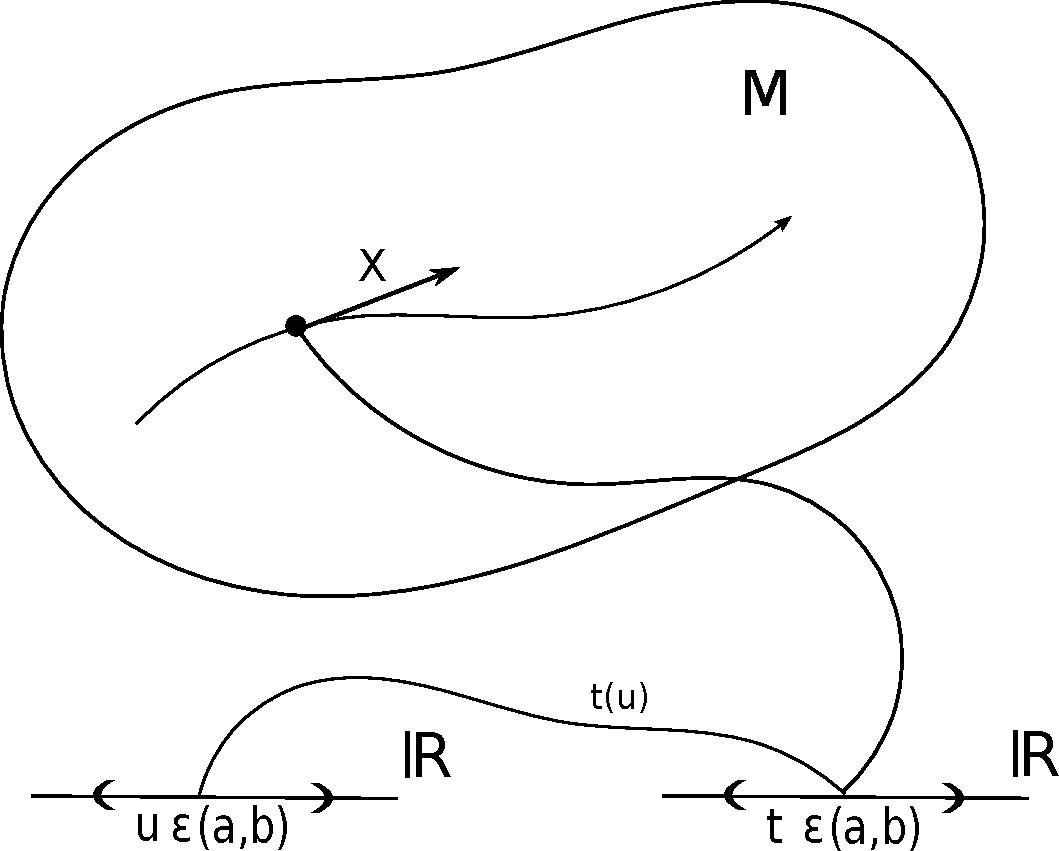
\includegraphics[width=0.7\textwidth]{Chapter 3/Figures/tdeu.pdf}
        \caption{Affine parameterization of the geodesics, here we illustrate the path (geodesic) a free particle will follow which is parameterized with a parameter $t$ but this is some application of the other parameter $u$.}
        \label{fig:tdeu}
    \end{figure}

    \begin{equation}
        Y = hX\;,\; h = \frac{dt}{du},
    \end{equation}

    \begin{equation}
        \Vec{\nabla}_YY=\Vec{\nabla}_{hX}(hX) = h\Vec{\nabla}_X(hX) = h^2\Vec{\nabla}_XX+hX = h^2\Vec{\nabla}_XX + hX\Vec{\nabla}_Xh,
    \end{equation}

    \begin{equation}
        \Vec{\nabla}_YY = hX\Vec{\nabla}_Xh = fY.
    \end{equation}

    Then we can see it is not parameterized affinely, the affine parameters are linear relations with the other parameters. Both are the same geodesic but the second one has not affine parameterization, but lets see how must be $h$ to have such a parameterization

    \begin{equation}
        X(h) = 0 \equiv x^{\alpha}\partial_{\alpha}h=0,
    \end{equation}

    therefore $h$ is covariantly constant and $\frac{dt}{du}=h$ or what is the same thing 

    \begin{equation}
        u = at + b\;, a>0.
    \end{equation}

    Where this is fulfilled $U$ is then either an affine parameter, thus its geodesics equation is

    \begin{equation}
        \Vec{\nabla}_YY = 0.
    \end{equation}

    In the general relativity the proper time $\tau$ is an affine parameters and it works to describe the time-like geodesics, \textit{the free particles move on geodesics} this having on count the Levi-Civita connection.

\section{Riemann's tensor}

        Here we're going to talk about the hearth of the general relativity, the hearth of the differential geometry (from a physical point of view hehe), the Riemann's tensor, inside this beautifull quantity there is the information of the curvature of our space-time the curvature of the geodesics? the curvature of the quantum vacuum? Yes, all this informations can be found inside this tensor, thus lets have fun on this topic.

    \subsection{Curvature of the Levi-Civita connection}

            Until here we haven't solved the problem of transporting a vector from a tangent space to another vector in another tangent space, here there is the solution of that, what is called the \textit{parallel transport}.\\

            Let $X$ a tangent vector to a curve, a tensor field $T$ is transported parallely along the curve if and only if

            \begin{equation}
                \Vec{\nabla}_XT=0.
            \end{equation}

            This means the tensor field does not change along the vector, therefore we had already solved the problem of parallel transport implicitly! $\Vec{\nabla}_XX=0$ this a curve whose tangent vector is parallely transported along the same curve, but but but, we need it to be unique, lets see if this is or not unique. Let $T$ be a tensor of rank $\binom{1}{1}$ we're going to define a coordinate chart such that

            \begin{equation}
                \phi = (x^1,...,x^n)\;X^{\mu}= \frac{d x^{\mu}}{d\lambda}
            \end{equation}

            where $\lambda$ is the curve parameter;

            \begin{equation}
                \left(\Vec{\nabla}_XT\right)^{\mu}_{\;\nu} = \left(X^{\sigma}\nabla_{\sigma}T^{\mu}_{\;\nu}\right) = X^{\sigma}\partial_{\sigma}T^{\mu}_{\;\nu} + \Gamma^{\mu}_{\;\rho\sigma}T^{\rho}_{\;\nu}X^{\sigma} - \Gamma^{\rho}_{\;\nu\sigma}T^{\mu}_{;\rho}X^{\sigma}
            \end{equation}

            \begin{equation}
                \left(\Vec{\nabla}_XT\right)^{\mu}_{\;\nu} = \frac{dx^{\sigma}}{d\lambda}\partial_{\sigma}T^{\mu}_{\;\nu} + \Gamma^{\mu}_{\;\rho\sigma}T^{\rho}_{\;\nu}X^{\sigma} - \Gamma^{\rho}_{\;\nu\sigma}T^{\mu}_{\;rho}X^{\sigma}=0.
            \end{equation}

            We have then a first order equation of the form

            \begin{equation}
                \frac{d T^{\mu}_{\;\nu}}{d\lambda}+... = 0,
            \end{equation}

            therefore there is a unique solution once we define the initial condition, then the tensor fields in $q$ and $p$ are isomorphic.

            \begin{myDef}
                The tensor of curvature of Riemann of a connection $\lambda$ is defined by

                \begin{equation}
                    R^a_{bcd}Z^bX^cY^d = \left(R\left(X,Y\right) Z\right)^a,
                \end{equation}

                where $X,Y,Z$ are vector fields and $R\left(X,Y\right)Z$ is also a vector field defined by

                \begin{equation}
                    R\left(X,Y\right)Z = \Vec{\nabla}_X\Vec{\nabla}_YZ - \Vec{\nabla}_Y\Vec{\nabla}_XZ - \Vec{\nabla}_{[X,Y]}Z.
                \end{equation}
            \end{myDef}

            The Riemann's tensor has te following properties

            \begin{enumerate}
                \item $R(X,Y)Z = - R(Y,X)Z$.

                \item 
                \begin{align}
                    R(fX,Y)Z = \Vec{\nabla}_{fX}\Vec{\nabla}_YZ - \Vec{\nabla}_Y\Vec{\nabla}_{fX}Z - \Vec{\nabla}_{[fX,Y]}Z\\
                    = f\Vec{\nabla}_X\Vec{\nabla}_YZ-\Vec{\nabla}_Y\left(f\Vec{\nabla}_XZ\right) - \Vec{\nabla}_{f[X,Y]-Y(f)X}Z\\
                    = f\Vec{\nabla}_X\Vec{\nabla}_YZ-f\Vec{\nabla}_Y\Vec{\nabla}_XZ - Y(f)\Vec{\nabla}_XZ - f\Vec{\nabla}_{[x,Y]}Z + Y(f)\Vec{\nabla}_XZ = fR(X,Y)Z. 
                \end{align}

                This means the Riemann's curvature tensors is multilinear in his two arguments, the demonstrations for the second argument is trivial therefore.

                \begin{equation}
                    R(X,fY)Z = fR(X,Y)Z.
                \end{equation}

                \item  \begin{align*}
                    R(X,Y)fZ = \Vec{\nabla}_X\Vec{\nabla}_Y(fZ) - \Vec{\nabla}_Y\Vec{\nabla}_X(fZ) - \Vec{\nabla}_{X,Y}fZ\\
                    = f\Vec{\nabla}_X\Vec{\nabla}_YZ - f\Vec{\nabla}_Y\Vec{\nabla}_XZ + \Vec{\nabla}_XZ\Vec{\nabla}_Yf + \Vec{\nabla}_Xf\Vec{\nabla}_YZ + Z\Vec{\nabla}_X\Vec{\nabla}_Yf\\
                    - \Vec{\nabla}_YZ\Vec{\nabla}_Xf - \Vec{\nabla}_Yf\Vec{\nabla}_XZ - Z\Vec{\nabla}_Y\Vec{\nabla}_Xf - \Vec{\nabla}_{{X,Y}}fZ\\
                    = f\left(\Vec{\nabla}_X\Vec{\nabla}_YZ - \Vec{\nabla}_Y\Vec{\nabla}_XZ - f\Vec{\nabla}_{{X,Y}}Z\right),
                \end{align*}

                \begin{equation}
                    R(X,Y)fZ = fR(X,Y)Z.
                \end{equation}
            \end{enumerate}

            In this way, the Riemann's tensor fulfills all those properties and correctly it defines a tensor, lets see how looks the Riemann's tensor given a coordinate chart and a basis $\{\mathbf{e}_{\mu}=\frac{\partial}{\partial x^{\mu}}\}$ and assuming a free of torsion theory

            \begin{equation}
                [\mathbf{e}_{\mu},\mathbf{e}_{\nu}]=0\;,
            \end{equation}

            \begin{equation}
                R(\mathbf{e}_{\rho},\mathbf{e}_{\sigma})\mathbf{e}_{\mu} = \Vec{\nabla}_{\mathbf{e}_{\rho}}\Vec{\nabla}_{\mathbf{e}_{\sigma}}\mathbf{e}_{\mu} - \Vec{\nabla}_{\mathbf{e}_{\sigma}}\Vec{\nabla}_{\mathbf{e}_{\rho}}\mathbf{e}_{\mu},
            \end{equation}

            \begin{align*}
                R(\mathbf{e}_{\rho},\mathbf{e}_{\sigma}) = \Vec{\nabla}_{\mathbf{e}_{\rho}}\left(\Gamma^{\tau}_{\;\mu\sigma} \mathbf{e}_{\tau}\right) - \Vec{\nabla}_{\mathbf{e}_{\tau}}- \Vec{\nabla}_{\mathbf{e}_{\sigma}}\left(\Gamma^{\tau}_{\;\rho\mu} \mathbf{e}_{\tau}\right)\\
                = \Vec{\nabla}_{\mathbf{e}_{\rho}}\Gamma^{\tau}_{\;\mu\sigma}\mathbf{e}_{\tau} + \Gamma^{\tau}_{\;\mu\sigma}\Vec{\nabla}_{\mathbf{e}_{\rho}}\mathbf{e}_{\tau} - \Vec{\nabla}_{\mathbf{e}_{\sigma}}\Gamma^{\tau}_{\;\rho\mu}\mathbf{e}_{\tau}-\Gamma^{\tau}_{\;\rho\mu}\Vec{\nabla}_{\mathbf{e}_{\sigma}}\mathbf{e}_{\tau},
            \end{align*}

            \begin{align*}
                R(\mathbf{e}_{\rho},\mathbf{e}_{\sigma}) \mathbf{e}_{\mu} = \partial_{\rho}\Gamma^{\tau}_{\;\mu\sigma}\mathbf{e}_{\tau} + \Gamma^{\tau}_{\;\mu\sigma}\Gamma^{\nu}_{\;\tau\rho}\mathbf{e}_{\nu} - \partial_{\sigma}\Gamma^{\tau}_{\;\mu\rho}\mathbf{e}_{\tau}-\Gamma^{\tau}_{\;\mu\rho}\Gamma^{\nu}_{\;\sigma\tau}\mathbf{e}_{\nu}\\
                = \left\{\partial_{\rho}\Gamma^{\nu}_{\;\mu\sigma} + \Gamma^{\tau}_{\;\mu\sigma}\Gamma^{\nu}_{\;\tau\rho}-\partial_{\sigma}\Gamma^{\tau}_{\;\mu\rho} - \Gamma^{\tau}_{\;\mu\rho}\Gamma^{\nu}_{\;\sigma\tau} \right\}\mathbf{e}_{\nu},
            \end{align*}

            \begin{equation}
                R^{\nu}_{\;\mu\rho\sigma} = \partial_{\rho}\Gamma^{\nu}_{\;\mu\sigma} + \Gamma^{\tau}_{\;\mu\sigma}\Gamma^{\nu}_{\;\tau\rho}-\partial_{\sigma}\Gamma^{\tau}_{\;\mu\rho} - \Gamma^{\tau}_{\;\mu\rho}\Gamma^{\nu}_{\;\sigma\tau}.
            \end{equation}

            \begin{myDef}
                The Ricci's curvature tensor, is a tensor of rank $\binom{0}{2}$ is defined by

                \begin{equation}
                    R_{ab}=R^c_{\;acb}.
                \end{equation}
            \end{myDef}

            With this tensor we can construct the Einstein's field equations, under the assumption of a free of torsion theory, and we can define the \textit{Ricci's identity} as

            \begin{equation}
                R^a_{\;bcd}Z^b = \Vec{\nabla}_c\Vec{\nabla}_dZ^a - \Vec{\nabla}_d\Vec{\nabla}_cZ^a,
            \end{equation}

            lets prove it

            \begin{align*}
                \left[R(X,Y)Z\right]^a = X^c\Vec{\nabla}_c\left(Y^d\Vec{\nabla}_dZ^a \right) - Y^d\Vec{\nabla}_d\left(X^c\Vec{\nabla}_cZ^a \right) - [X,Y]^c\Vec{\nabla}_cZ^a\\
                = X^cY^d\Vec{\nabla}_c\Vec{\nabla}_dZ^a + X^c\left(\Vec{\nabla}_cY^d\right)\Vec{\nabla}_dZ^a - Y^dX^c\Vec{\nabla}_d\Vec{\nabla}_cZ^a - Y^d\left(\Vec{\nabla}_dX^c \right)\Vec{\nabla}_cZ^a-[X,Y]^c\Vec{\nabla}_cZ^a,
            \end{align*}

            \begin{equation}
                \left[R(X,Y)Z \right]^a = X^cY^d\left[\Vec{\nabla}_c\Vec{\nabla}_dZ^a - \Vec{\nabla}_d\Vec{\nabla}_cZ^a \right] + X^c\left(\Vec{\nabla}_cY^d \right)\Vec{\nabla}_dZ^a - Y^d\left(\Vec{\nabla}_dX^c\right)\Vec{\nabla}_cZ^a - [X,Y]^c\Vec{\nabla}_cZ^a.
            \end{equation}

            and for a free of torsion theory we can develop the commutator

            \begin{equation}
                [X,Y]^c = \left[\Vec{\nabla}_XY - \Vec{\nabla}_YX \right]^c = X^e\Vec{\nabla}_eY^c - Y^e\Vec{\nabla}_eX^c,
            \end{equation}

            \begin{equation}
                [X,Y]\Vec{\nabla}_cZ^a = X^e\left(\Vec{\nabla}_eY^c \right)\left(\Vec{\nabla}_cZ^a\right) - Y^e\left(\Vec{\nabla}_eY^c \right)\left(\Vec{\nabla}_cZ^a\right),
            \end{equation}

            \begin{equation}
                X^c\left(\Vec{\nabla}_cY^d \right)\left(\Vec{\nabla}_dZ^a\right)-Y^d\left(\Vec{\nabla}_dX^c\right)\left(\Vec{\nabla}_cZ^a\right) - [X,Y]c\Vec{\nabla}_CZ^a = 0,
            \end{equation}

            \begin{equation}
                \left[R(X,Y)Z \right]^a = \left(\Vec{\nabla}_c\Vec{\nabla}_dZ^a - \Vec{\nabla}_d\Vec{\nabla}_cZ^a \right)X^cY^d = R^a_{\;bcd}Z^bX^cY^d.
            \end{equation}

            By comparation it only rests that

            \begin{equation}
                \Vec{\nabla}_c\Vec{\nabla}_dZ^a - \Vec{\nabla}_d\Vec{\nabla}_cZ^a = R^a_{\;bcd}Z^b.
            \end{equation}

            \begin{figure}[h]
                \centering
                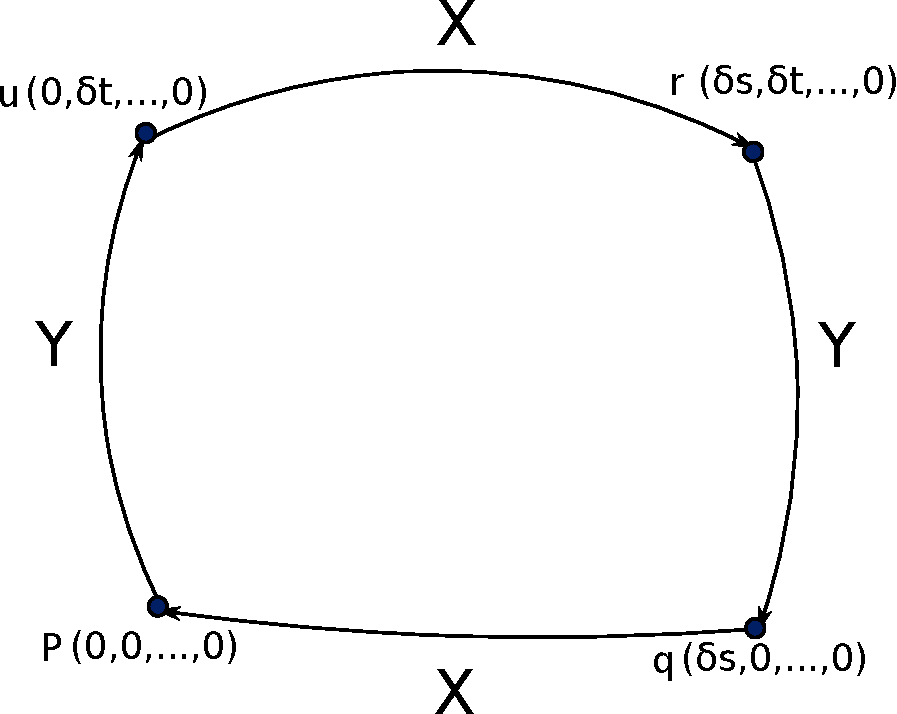
\includegraphics[width=0.6\textwidth]{Chapter 3/Figures/Tareinha.pdf}
                \caption{Connection between $q$ and $p$ with a curve along a variation of $s$ with $X$ as tangent vector, in the same way $q$ and $r$ can be connected by a curve with $Y$ as tangent vector, $p$ and $u$ can be connected with a curve with $Y$ as tangent vector and same with $u$ and $r$ but with $X$ as tangent vector.}
                \label{fig:tareinha}
            \end{figure}

            Now, lets turn back to the relation between the Riemann's tensor and the dependence of the path of the parallel transport. Let $X$ and $Y$ vector fields which are linearly independent everywhere such that $[X,Y]=0$. Let $(s,t,...)$ a coordinate chart such that

            \begin{equation}
                X=\frac{\partial}{\partial s}\;\&\;Y = \frac{\partial}{\partial t}.
            \end{equation}

            Let $p\in M$ and given a coordinate chart $p$ is represented as $(0,...,0)$. Let $q,r,u$ points with coordinates $(\delta s,0,0,...)$, $(\delta s,\delta t, 0,...)$, $(0,\delta L,0,...)$, respectively, where $\delta s$, $\delta t$ are little displacement of that coordinate, we can connect the fourth point as is illustrated in the figure \ref{fig:tareinha}.\\

            Now, let $Z_p \;\in\;T_p(M)$.  Lets transport parallely $Z_p$ along $pqr$ to obtain a vector $Z_r \;\in\; T_r(M)$, the same thing but to transport $Z_p$ along $pur$ to obtain the vector $Z_r'\;\in\;T_r(M)$ and lets calculate the difference $Z_r'-Z_r$ for a free of torsion connection. it is convenient to introduce a new coordinate chart known as \textit{normal coordinates} in $p$, ($\Gamma^{\mu}_{\;\nu\rho}(p)=0$). The indices $\mu,\nu$ will refer to this chart. $S$ and $t$ will be used as parameters along the curves whose tangent vectors are $X$ and $Y$ ,respectively. \\

            $pq$ is an integral curve whose tangent vector is $X$ and parameter $S$. Along of $pq$, $Z$ is transported parallely: $\Vec{\nabla}_XZ=0,$ therefore

            \begin{equation}
                \frac{d Z^{\mu}}{ds} = - \Gamma^{\mu}_{\;\nu\rho}Z^{\nu}X^{\rho},
            \end{equation}

            and in this way

            \begin{equation}
                \frac{d^2Z^{\mu}}{ds^2} = - \left(\Gamma^{\mu}_{\;\nu\rho}Z^{\nu}X^{\rho} \right)_{,\sigma}X^{\sigma}.
            \end{equation}

            Now using Taylor's expansion theorem we get:

            \begin{equation}
                Z^{\mu}_q = Z^{\mu}_q + \left(\frac{dZ^{\mu}}{ds} \right)_p\delta s + \frac{1}{2}\left(\frac{d^2Z^{\mu}}{ds^2} \right)_p\delta s^2 + \mathcal{O}(\delta s^3).
            \end{equation}

            We must note that:

            \begin{equation}
                \frac{d^2Z^{\mu}}{ds^2}=-\Gamma^{\mu}_{\;\nu\rho,\sigma}Z^{\nu}X^{\rho}X^{\sigma} - \Gamma^{\mu}_{\;\nu\rho}Z^{\nu}_{\;,\sigma}X^{\rho}X^{\sigma} - \Gamma^{\mu}_{\;\nu\rho}Z^{\nu}X^{\rho}_{\;,\sigma}X^{\sigma},
            \end{equation}

            \begin{equation}
                Z^{\mu}_q = Z^{\mu}_p - \frac{1}{2}\left(\Gamma^{\mu}_{\;\nu\rho,\sigma}Z^{\nu}X^{\rho}X^{\sigma} \right)_p\delta s^2 + \mathcal{O}(\delta s^3),
            \end{equation}

            where we had used $\Gamma^{\mu}_{\;\nu\rho}(p)=0$ in normal coordinates at $p.$Now consider the parallel transport along $qr$:


            \begin{align}
                \frac{dZ^{\mu}}{dt} = -\Gamma^{\mu}_{\;\nu\rho}Z^{\nu}Y^{\rho},\\
                \frac{d^2Z^{\mu}}{dt^2} = - \left(\Gamma^{\mu}_{\;\nu\rho}Z^{\nu}Y^{\rho} \right)_{,\sigma}Y^{\sigma,}
            \end{align}

            \begin{equation}
                Z^{\mu}_r = Z^{\mu}_q - \left(\Gamma^{\mu}_{\;\nu\rho}Z^{\nu}Y^{\rho} \right)_q\delta t - \frac{1}{2}\left[\left(\Gamma^{\mu}_{\;\nu\rho}Z^{\nu}Y^{\rho} \right)_{,\sigma}Y^{\sigma} \right]_q\delta t^2 + \mathcal{O}(\delta t^3).
            \end{equation}

            

            \begin{align}
                \left(\Gamma^{\mu}_{\;\nu\rho}Z^{\nu}Y^{\rho} \right)_Q = \left(\Gamma^{\mu}_{\;\nu\rho}Z^{\nu}Y^{\rho} \right)_p + \left[\frac{d}{ds}\left(\Gamma^{\mu}_{\;\nu\rho}Z^{\nu}Y^{\rho} \right) \right]_p\delta s + \mathcal{O}(\delta S^2)\\
                = \left[\left(\Gamma^{\mu}_{\;\nu\rho}Z^{\nu}Y^{\rho} \right)_{,\sigma} X^{\sigma}\right]_p\delta s + \mathcal{O}(\delta s^2)\\
                = \left(\Gamma^{\mu}_{\;\nu\rho}z^{\nu}Y^{\rho}X^{\sigma} \right)_p\delta s + \mathcal{O}(\delta s^2)
            \end{align}

            \begin{equation}
                \left[\left(\Gamma^{\mu}_{\;\nu\rho}Z^{\nu}Y^{\rho} \right)_{,\sigma} \right]_q = \left[\left(\Gamma^{\mu}_{\;\nu\rho}Z^{\nu}Y^{\rho} \right)_{,\Sigma}Y^{\sigma} \right]_p + \mathcal{O}(\delta s) = \left(\Gamma^{\mu}_{\;\nu\rho,\sigma}Z^{\nu}Y^{\rho}Y^{\sigma} \right)_p + \mathcal{O}(\delta s),
            \end{equation}

            \begin{equation}
                Z^{\mu}_r = Z^{\mu}_q - \left[\left(\Gamma^{\mu}_{\;\nu\rho}Z^{\nu}Y^{\rho}X^{\sigma} \right)_p \delta s + \mathcal{O}(\delta s^2)\right]\delta t - \frac{1}{2}\left[\left(\Gamma^{\mu}_{\;\nu\rho}Z^{\nu}Y^{\rho}X^{\sigma} \right)_p \delta s + \mathcal{O}(\delta s^2) \right]\delta t^2 + \mathcal{O}(\delta t^2),
            \end{equation}

            \begin{equation}
                Z^{\mu}_r = Z^{\mu}_p - \frac{1}{2}\left(\Gamma^{\mu}_{\;\nu\rho,\sigma} \right)_p\left[Z^{\nu}\left(X^{\rho}X^{\sigma}\delta s^2 + Y^{\rho}Y^{\sigma}\delta t^2  + 2Y^{\rho}X^{\sigma}\delta s\delta t \right)\right]_p + \mathcal{O}(\delta ^3).
            \end{equation}

            Now, consider the parallel transport along $pur$. The result can be obtained from the last expression interchanging $X$ with $Y$ and $s$ with $t$

            \begin{equation}
                Z'^{\mu}_r = Z^{\mu}_p-\frac{1}{2}\left(\Gamma^{\mu}_{\;\nu\rho,\sigma} \right)_p\left[Z^{\nu}\left(Y^{\rho}Y^{\sigma}\delta t^2 + X^{\rho}X^{\sigma}\delta s^2 + 2X^{\rho}Y^{\sigma}\delta t \delta s \right) \right]_p + \mathcal{O}(\delta^3)
            \end{equation}

            in this way the difference between the two parallel transport is

            \begin{align}
                \triangle Z^{\mu}_r = Z'^{\mu}_r - Z^{\mu}_r\\
                = \left[\Gamma^{\mu}_{\;\nu\rho,\sigma}Z^{\nu}\left(Y^{\rho}X^{\sigma} - x^{\rho}Y^{\sigma} \right) \right]_p\delta t \delta s + \mathcal{O}(\delta^3)\\
                = \left[\left(\Gamma^{\mu}_{\;\nu\sigma,\rho} - \Gamma^{\mu}_{\;\nu\rho,\sigma} \right)Z^{\nu}X^{\rho}Y^{\sigma} \right]_p\delta s \delta t 
                 \mathcal{O}(\delta^3)\\
                 = \left[\left(R^{\mu}_{\;\nu\rho\sigma} - \Gamma^{\tau}_{\;\nu\sigma}\Gamma^{\mu}_{\;\tau\rho} + \Gamma^{\tau}_{\;\nu\rho}\Gamma^{\mu}_{\;\tau\sigma} \right)Z^{\nu}X^{\rho}X^{\sigma} \right]_p\delta t \delta s + \mathcal{O}(\delta^3),
            \end{align}

            \begin{align}
                \triangle Z^{\mu}_r = \left(R^{\mu}_{\;\nu\rho\sigma}Z^{\nu}X^{\rho}X^{\sigma} \right)_p\delta s \delta t + \mathcal{O}(\delta^3),\\
                \triangle Z^{\mu}_r = \left(R^{\mu}_{\;\nu\rho\sigma}Z^{\nu}X^{\rho}X^{\sigma} \right)_r\delta s \delta t + \mathcal{O}(\delta^3).
            \end{align}

            In the last equality is used that the quantities in $p$ and $r$ are different by $\mathcal{O}(\delta)$. this result is derived in a coordinate basis defined using normal coordinates in $p$ but now both side take on count tensors in $r$ therefore our equations is independent of the basis, thus

            \begin{equation}
                \left(R^a_{\;bcd}Z^bX^cY^d \right)_r = \lim_{\delta \to 0} \frac{\triangle Z^{\mu}_r}{\delta s \delta t}.
            \end{equation}

            \textit{The Riemmann's tensor measures the dependence of the path of the parallel transport.} The last result can be reinterpreted describing the effect of the parallel transport of a vector $Z^a_r$ along a closed curved $qpur$ , see figure \ref{fig:tareinha}, to obtain the vector $Z'^a_r$. In this way $\triangle Z^a_r$ measures the change in $Z^a_r$ when it is transported parallel y around a closed curve.\\
            
            Lets see the symmetries of the Riemann's tensor

            \begin{enumerate}
                \item $R^a_{\;bcd} = - R^a_{\;bdc}$ it is anti symmetric.

                \item If $\vec{\nabla}$ is a free of torsion connections then

                \begin{equation}
                    R^a_{\;[bcd]} = \frac{1}{3!}\left(R^a_{\;bcd} + R^a_{\;cdb} + R^a_{\;dbc}- R^a_{\;cbd} - R^a_{\;bdc} - R^a_{\;dcb}\right) = 0.
                \end{equation}

                \item  If $\Vec{\nabla}$is a free of torsion connection then
                \begin{equation}
                    R^a_{\;b[cd;e]}=0.
                \end{equation}
            \end{enumerate}

            Thanks to the fact the metric tensor is covariantly constant, then it will allow us to raise and low indices and using these we can see the following properties

            \begin{enumerate}
                \item $R_{abcd}=R_{cdab}$.
                \item $R_{ab}=R_{ba}$.
            \end{enumerate}

            \begin{myDef}
                The Ricci's scalar is 

                \begin{equation}
                    R = g^{ab}R_{ab}.
                \end{equation}
            \end{myDef}

            \begin{myDef}
                The Einstein's tensor, is a symmetric tensor of rank $\binom{0}{2}$ and is defined as

                \begin{equation}
                    G_{ab}=R_{ab}-\frac{1}{2}g_{ab}R.
                \end{equation}
            \end{myDef}

            \textbf{Proposition:} the covariant derivative of the Einstein's tensor is zero

            \begin{equation}
                \Vec{\nabla}_aG^{ab}=0.
            \end{equation}

            \textbf{Demonstration}:

            \begin{align*}
                \Vec{\nabla}_aG^{ab} = \Vec{\nabla}_a\left[R^{ab} - \frac{1}{2}g^{ab}R \right] = \Vec{\nabla}_aR^{ab}-\frac{1}{2}\Vec{\nabla}_ag^{ab}R - \frac{1}{2}g^{ab}\Vec{\nabla}_aR\\
                = \Vec{\nabla}_aR^{ab}-\frac{1}{2}\Vec{\nabla}_ag^{ab}\left(g^{cd}R_{cd} \right) - \frac{1}{2}g^{ab}\left[\Vec{\nabla}_ag^{cd}R_{cd} + g^{cd}\Vec{\nabla}_aR_{cd} \right]\\
                =\Vec{\nabla}_aR^{ab}-\frac{1}{2}\Vec{\nabla}_ag^{ab}\left(g^{cd}R_{cd} \right) - \frac{1}{2}\Vec{\nabla}_ag^{cd}g^{ab}R_{cd} - \frac{1}{2}g^{ab}g^{cd}\Vec{\nabla}_aR_{cd}\\
                =\Vec{\nabla}_aR^{ab}-\frac{1}{2}\Vec{\nabla}_ag^{ab}\left(g^{cd}R_{cd} \right) - \frac{1}{2}\Vec{\nabla}_ag^{cd}g^{ab}R_{cd}-\frac{1}{2}g^{ab}g^{cd}\Vec{\nabla}_aR_{cd},
            \end{align*}

            and using the Leibniz rule is easy to see that

            \begin{equation}
                \Vec{\nabla}_a\left[g^{ab}g^{cd}R_{cd} \right] = \Vec{\nabla}_ag^{ab}\left[g^{cd}R_{cd} \right] + g^{ab}R_{cd}\Vec{\nabla}_ag^{cd} + g^{ab}g^{cd}\Vec{\nabla}_aR_{cd}      ,  \end{equation}

                thus

                \begin{equation}
                    \Vec{\nabla}_aG^{ab} = \Vec{\nabla}_aR^{ab} + \frac{1}{2}g^{ab}g^{cd}\Vec{\nabla}_aR_{cd} - \Vec{\nabla}_aR^{ab} - \frac{1}{2}g^{ab}g^{cd}\Vec{\nabla}_aR_{cd} = 0.
                \end{equation}

        \subsubsection{Einstein's equations}

            These equations holds under some postulates, the known as the general relativity postulates which are

            \begin{enumerate}
                \item The space-time is a pseudo-Riemannian manifold equiped with a Levi-Civita connection $(M,\mathbb{G},\Vec{\nabla})$.

                \item The free particles follows geodesics.

                \item The energy-momentum tensor $T_{ab}$ is conserved: $\Vec{\nabla}_aT^{ab}=0$.

                \item The Einstein's tensor satisfies  that

                \begin{equation}
                    G_{ab}=R_{ab}-\frac{1}{2}g_{ab}R = \frac{8\pi G}{C^4}T_{ab}.
                \end{equation}
            \end{enumerate}

            We can see that there is no matter thus $T_{ab}=0 \rightarrow R= 0 \rightarrow R_{ab}=0$ lets see this

            \begin{equation*}
                g^{ab}\left(R_{ab} - \frac{1}{2}g_{ab}R \right) = \alpha g^{ab}T_{ab},
            \end{equation*}

            \begin{equation*}
                R-2R = \alpha T \rightarrow T = -\frac{1}{\alpha}R,
            \end{equation*}

            \begin{equation}
                R_{ab} = \alpha T_{ab}+\frac{1}{2}g_{ab}R = \alpha\left(T_{ab}-\frac{1}{2}g_{ab}T \right),
            \end{equation}

            we can see easily that if there is no matter the Ricci's tensor is zero.\\

            The Einstein's equations are ten second order, non linear and copuled equations of the metric tensor, but this form is not unique. Lets think about a symmetric tensor $H_{ab}$, which is covariantly constant, the space-time must be a pseudo-Riemannian manifold of four dimensions, with a levi-civitta connections, thus by the \textbf{Lovelack theorem}

            \begin{equation}
                H_{ab}=\alpha G_{ab} + \beta g_{ab},
            \end{equation}

            \begin{equation}
                G_{\alpha\beta} + \Lambda g_{\alpha\beta} = \frac{8\pi G}{C^4}T_{\alpha\beta}.
            \end{equation}

            $\Lambda$ is known as the cosmologic constant and it was first rejected by Einstein but reintroduced by himself to explain the accelerated expansion of the universe, this constant is nowadays studied in relation with the dark energy and dark matter.

    \subsection{Properties related to the Riemann's tensor}

        In this part we're going to study tensor equations related to the Riemann's tensor and some really important identities as the Jacobi and Bianchi's identities, which are really important in the development of general relativity and will guide us to the Einstein's tensor. Let $\{\mathbf{e}_{\alpha}\} = \left\{\frac{\partial}{\partial x^{\alpha}} \right\}$ a coordinate basis , then in this basis the components of the Riemann's tensor become

        \begin{equation}
            R^{\alpha}_{\;\beta\mu\nu} = \partial_{\nu}\Gamma^{\alpha}_{\;\beta\nu} - \partial_{\nu}\Gamma^{\alpha}_{\;\beta\mu} + \Gamma^{\alpha}_{\;\sigma\mu}\Gamma^{\sigma}_{\;\beta\nu} - \Gamma^{\alpha}_{\;\sigma\nu}\Gamma^{\sigma}_{\;\beta\mu}.
        \end{equation}
        We're going to consider the components of the Riemann's tensor in a locally inertial reference frame known as \textit{normal coordinates}, these are special such that

        \begin{equation}
            \Gamma^{\alpha}_{\;\sigma\mu}(p)=0,\;\;\partial_{\mu}\Gamma^{\alpha}_{\;\beta\nu}(p)\neq0,
        \end{equation}

        from these point of view the Riemann's tensor takes the following form:

        \begin{equation}
            R^{\alpha}_{\;\beta\mu\nu}=\partial_{\mu}\Gamma^{\alpha}_{\;\beta\nu}-\partial_{\nu}\Gamma^{\alpha}_{\;\beta\mu},
        \end{equation}
        and we gotta calculate the Cristoffel's symbol, thus

        \begin{align*}
            \Gamma^{\alpha}_{\;\mu\nu}=\frac{1}{2}g^{\alpha\beta}\left(\partial_{\nu}g_{\beta\mu} + \partial_{\mu}g_{\beta\nu} - \partial_{\beta}g_{\mu\nu} \right).\\
            \partial_{\sigma}\Gamma^{\alpha}_{\;\mu\nu} = \frac{1}{2}g^{\alpha\beta}\left(\partial_{\sigma}\partial_{\nu}g_{\beta\mu} + \partial_{\sigma}\partial_{\mu}g_{\beta\nu} - \partial_{\sigma}\partial_{\beta}g_{\mu\nu} \right)\\
            + \frac{1}{2}\left(\partial_{\nu}g_{\beta\mu} + \partial_{\mu}g_{\beta\nu} - \partial_{\beta}g_{\mu\nu} \right)\partial_{\sigma}g^{\alpha\beta}
        \end{align*}

        \begin{equation}
            \partial_{\sigma}\Gamma^{\alpha}_{\;\mu\nu} = \frac{1}{2}g^{\alpha\beta}\left(\partial_{\sigma}\partial_{\nu}g_{\beta\mu} + \partial_{\sigma}\partial_{\mu}g_{\beta\nu} - \partial_{\sigma}\partial_{\beta}g_{\mu\nu} \right) + \frac{1}{2}\left[\beta,\mu\nu \right]\partial_{\sigma}g^{\alpha\beta},
        \end{equation}

        \begin{equation}\label{eq:CoordNorm}
            \partial_{\sigma}\Gamma^{\alpha}_{\;\mu\nu} = \frac{1}{2}g^{\alpha\beta}\left(\partial_{\sigma}\partial_{\nu}g_{\beta\mu} + \partial_{\sigma}\partial_{\mu}g_{\beta\nu} - \partial_{\sigma}\partial_{\beta}g_{\mu\nu} \right).
        \end{equation}
        
we're going to use the equation \ref{eq:CoordNorm}
on the Riemman's tensor on the point  $p \;\in\;M$  in the following way

\begin{align*}
R^{\alpha}_{\;\beta\mu\nu}|_p = \frac{1}{2}g^{\alpha\sigma}\left(\partial_{\mu}\partial_{\nu}g_{\sigma\beta} +\partial_{\mu}\partial_{\beta}g_{\sigma\nu} - \partial_{\mu}\partial_{\sigma}g_{\beta\nu} \right)|_p - \frac{1}{2}g^{\alpha\sigma}\left(\partial_{\nu}\partial_{\mu}g_{\sigma\beta} + \partial_{\nu}\partial_{\beta}g_{\sigma\mu} - \partial_{\mu}\partial_{\sigma}g_{\mu\beta} \right)|_p,
\end{align*}

\begin{equation}
    R^{\alpha}_{\;\beta\mu\nu}|_p = \frac{1}{2}g^{\alpha\sigma}\left(\partial_{\beta}\partial_{\mu}g_{\sigma\nu} - \partial_{\nu}\partial_{\beta}g_{\sigma\mu} + \partial_{\nu}\partial_{\sigma}g_{\mu\beta} - \partial_{\mu}\partial_{\sigma}g_{\beta\nu} \right)|_p,
\end{equation}

\begin{equation}
    R_{\alpha\beta\mu\nu}|_p = g_{\alpha\lambda}R^{\lambda}_{\;\beta\mu\nu} = \frac{1}{2} \left(\partial_{\beta}\partial_{\mu}g_{\alpha\nu} - \partial_{\nu}\partial_{\beta}g_{\alpha\mu} + \partial_{\nu}\partial_{\alpha} - \partial_{\mu}\partial_{\alpha}g_{\beta\nu} \right)|_p
\end{equation}

From here on we can see the following relations, which are tensor equations and do not depend on the coordinate chart

\begin{align}
    R_{\alpha\beta\mu\nu}=-R_{\beta\alpha\mu\nu},\\
    R_{\alpha\beta\mu\nu}=-R_{\alpha\beta\nu\mu},\\
    R_{\alpha\beta\mu\nu}R_{\mu\nu\alpha\beta},\\
    R_{\alpha\beta\mu\nu}+R_{\alpha\nu\beta\mu}+R_{\alpha\mu\nu\beta} = R_{\alpha[\beta\mu\nu]}=0.
\end{align}

These relations and symmetries on the Riemann's tensor will allow us to reduce a system of 256 equations to 18 equations. There are more relations beyond theses, the known as the \textit{Bianchi identities} which will be worth to define and arrive the Einstein's tensor. In normal coordinates we have got

\begin{equation}
    \Vec{\nabla}_{\lambda}R_{\alpha\beta\mu\nu}=\partial_{\lambda}R_{\alpha\beta
    \mu\nu}= \frac{1}{2}\left(\partial_{\lambda}\partial_{\beta}\partial_{\mu}g_{\alpha\nu}  - \partial_{\lambda}\partial_{\nu}\partial_{\beta}g_{\alpha\mu} + \partial_{\lambda}\partial_{\nu}\partial_{\alpha}g_{\mu\beta} - \partial_{\lambda}\partial_{\mu}\partial_{\alpha}g_{\beta\nu}\right)|_p,
\end{equation}

We can find an analogous to the Jacobi's identity with covariant derivatives

\begin{align}
    \Vec{\nabla}_{\lambda}R_{\alpha\beta\mu\nu} + \Vec{\nabla}_{\nu}R_{\alpha\beta\lambda\mu} + \Vec{\nabla}_{\mu}R_{\alpha\beta\nu\lambda}=0,\\
    R_{\alpha\beta\left[\mu\nu;\lambda \right]} = \Vec{\nabla}_{[\lambda}R_{\mu\nu]\alpha\beta}=0.
\end{align}

All this geometrical developement was done by Riemann with the intention of generalizing the Gauss work on curvature. Lets find out the contracted Bianchi's identities, therefore

\begin{equation}
    \left[\Vec{\nabla}_eR_{abbcd} + \Vec{\nabla}_dR_{abec} + \Vec{\nabla}_cR_{abde} = 0 \right]g^{ac},
\end{equation}

\begin{equation}
    \Vec{\nabla}_eR_{bd} + \Vec{\nabla}_d\left(g^{ac}R_{abec} \right) + g^{ac}\Vec{\nabla}_cR_{abdc}=0,
\end{equation}

\begin{equation}
    \Vec{\nabla}_eR_{bd} - \Vec{\nabla}_dR_{be} + \Vec{\nabla}^aR_{abde}=0,
\end{equation}

\begin{equation}\label{eq:PrimerContraida}
    \Vec{\nabla}_eR_{bd} - \Vec{\nabla}_dR_{be}+\Vec{\nabla}^aR_{abde}=0.
\end{equation}

From the Bianchi's identity for the Riemann's tensor we've found the repective identity for the Ricci's tensor also known as the \textit{contracted Bianchi identity} given in the equations \ref{eq:PrimerContraida} but we can contract it one more time and obtaint the Bhianchi identity for the Ricci's scalar wich is related with the Einstein's tensor and also is a clue to the Einstein's equations, so contracting the equation \ref{eq:PrimerContraida} we'll then have

\begin{equation}
    g^{bd}\left[\Vec{\nabla}_eR_{bd}-\Vec{\nabla}_dR_{be} + \Vec{\nabla}^aR_{abde} = 0\right],
\end{equation}

\begin{equation}
    \Vec{\nabla}_eR-\Vec{\nabla}^bR_{be}-\Vec{\nabla}^aR_{ae}=0,
\end{equation}

\begin{equation}\label{eq:Bhianchitwice}
    \Vec{\nabla}^aR_{ae}=\frac{1}{2}\Vec{\nabla}_eR.
\end{equation}

The equation \ref{eq:Bhianchitwice} is known as the Bianchi's identity twice contracted and playing a bit with this equations we will find something special, lets find out it

\begin{align*}
    \Vec{\nabla}^aR_{ae}-\frac{1}{2}\Vec{\nabla}_eR=0,\\
    \Vec{\nabla}^aR_{ae}\frac{1}{2}g_{ae}\Vec{\nabla}^aR=0,\\
    \Vec{\nabla}^a\left(R_{ae}-\frac{1}{2}g_{ae}R \right)=0,
\end{align*}

\begin{equation}
    \Vec{\nabla}^aG_{ab}=0\;\;;\;\;G_{ab}=R_{ab}-\frac{1}{2}g_{ab}R,
\end{equation}

Thehre appers naturally the Einstein's tensor! Now, in the curved spaces the geodesics aren't always parallel there are some separation between one or another geodesic but how can we measure or have an idea of how far or deviated is a geodesic from other.

\subsection{Geodesic deviation}

    \begin{myDef}
        Let $M$ a manifold with a Levi-Civita connection $\Vec{\nabla}$ . A monoparametric family of geodesics is a map

        \begin{equation}
            \gamma\;:\;I \times I' \rightarrow M,
        \end{equation}
        where $I$, $I'$ are two open intervals on the $\mathbb{R}$ such that

        \begin{enumerate}
            \item For a $S$ constant, $\gamma(s,t)=\gamma_s(t)$ is a geodesic with affine parameters $t$, therefore $S$ would be a parameter that tags the geodesic.
            \item The collection of these curves define a $2D$ smooth surface and is a subset of the manifold $\Sigma \subset M$ as is represented in the figure \ref{fig:GeodesicDeviation}
        \end{enumerate}

    \begin{figure}[h]
        \centering
        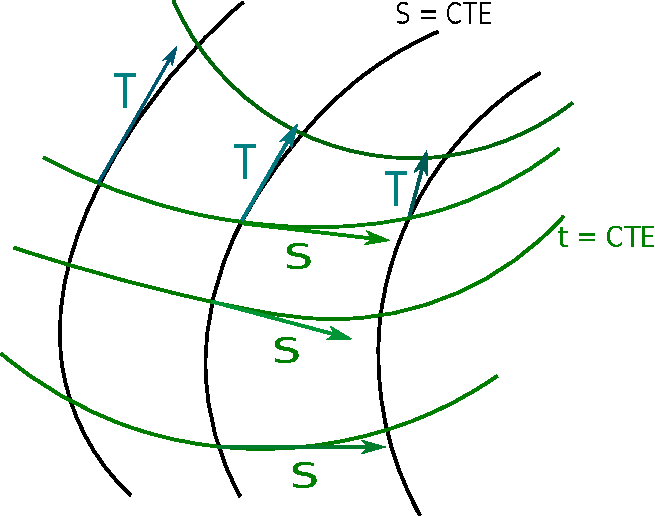
\includegraphics[width=0.75\linewidth]{Chapter 3/Figures/GeodesicDeviation.pdf}
        \caption{Representation of all the possible subsets of $S$ constant and $t$ constant, this is an analogous to what is done in the formulation $3+1$ where we separate the space-time and folds as a Cauchy space. }
        \label{fig:GeodesicDeviation}
    \end{figure}
    \end{myDef}
To quantify the deviation between to adjacent geodesics, lets first, suppose a coordinate chart $x^{\mu}(s,t)\in M$, therefore

    \begin{equation}
        T^{\mu}=\frac{\partial x^{\mu}}{\partial t},\;\; S^{\mu} = \frac{\partial x^{\mu}}{\partial s}.
    \end{equation}

    The first vectors $T^{\mu}$ are called the tangent vectors to the geodesics, and the other ones $S^{\mu}$ are named the deviation vectors. We're going to express the vectors of the chart in terms of the vectors of deviation.

    \begin{equation}
        x^{\mu}(s+\delta s,t) = x^{\mu}(s,t) + \left(\frac{\partial x^{\mu}}{\partial s} \right)\delta s + \mathcal{O}(\delta s^2).
    \end{equation}
We're going to analyze the vector $S$ and its changing along the geodesic $T$.  To do it, we can define a relative speed between geodesics

\begin{equation}
    V^a=\left(\Vec{\nabla}_TS \right)^a = T^b\Vec{\nabla}_bS^a,
\end{equation}

if we can talk about the relative speed between geodesics, we can also talk about the acceleration relative between geodesics, then

\begin{equation}
    a^a = \left(\nabla_TV \right)^a = T^b\Vec{\nabla}_bV^a = T^c\Vec{\nabla}_c\left(T^b\Vec{\nabla}_bS^a \right) = a^a = \Vec{\nabla}_T\Vec{\nabla}_TS^a,
\end{equation}

we can introduce the coordinate basis on $\Sigma$ as $S = \partial_s$ and $T=\partial_t$  and because we're having a theory free of torsion so from the commutator we have

\begin{equation}
    \left[T,S \right](f) = T[S(f)] - S[T(f)] = \partial_t[S(f)] - \partial_s[T(f)]=0,
\end{equation}

under these conditions and without torsion then

\begin{equation}
    \Vec{\nabla}_TS=\Vec{\nabla}_ST\rightarrow T^b\nabla_bS^a=S^b\nabla_bT^a,
\end{equation}
\begin{equation}\label{eq:CasiAcc}
    \Vec{\nabla}_T\Vec{\nabla}_TS=R(T,S)T.
\end{equation}

Using \ref{eq:CasiAcc} into the acceleration relative into geodesics, then we have

\begin{equation}
    a^a = [\Vec{\nabla}_T\Vec{\nabla}_TS]^a = \left(R(T,S)T \right)^a = R^a_{\;bcd}T^bT^cS^d,
\end{equation}

\begin{equation}\label{eq:AccelerationRiemann}
    a^a = R^a_{\;bcd}T^bT^cS^d.
\end{equation}

The equation \ref{eq:AccelerationRiemann} implies something really, reallly amazing and important \textbf{\textit{The acceleration is curvature}} but we gotta read this equations correctly, as cause and effect, the presence of curvature produces and effect we call acceleration, we can denotate the equation \ref{eq:AccelerationRiemann} in other way, as

\begin{equation}
    a^a = \frac{D^2}{Dt^2}S^a = R^a_{\;bcd}T^bT^cS^d.
\end{equation}
    
\section{Gravitation and the Einstein's field equation}

    We have found a relation between the curvature tensor and the relative acceleration between geodesics, and knowing a particle test has a geodesics as a path, then different curvatures produces different accelerations, and from the experiments we've talk about in the first part acceleration is indistinguishable from gravity.\\
    Well then, how are going to relate the acceleration to curvature? To do this, we're going to solve the Einsteins field equations in the Newtonian limit to interpret this physically and see if the Newton's theory was plane or curved of if it was, from the beginning a geometrical theory. First we're going to set some properties of the manifolds to set the space-time and use it to develop this theory.

    \begin{enumerate}
        \item The set of all the events in a $4D$ manifold with pseudo-Riemannian metric and a Levi-Civita connections is a differential manifold called \textit{space-time} denoted by $(M,\mathbb{G},\Vec{\nabla})$.
        \item The Manifold is Lorentzian.
        \item The weak equivalence principle is fulfilled.
        \item The Einstein's equivalence principle  is fulfilled.
    \end{enumerate}
    \subsection{Newtonian limit}

    We gotta then talk about particles whose speed is a lot less than the speed of light $C$  and the gravitational field is stationary and weak, using geometrical coordinates $C=1$ then

    \begin{equation}
        \frac{d\Vec{X}}{d\tau} \ll \frac{dt}{d\tau},
    \end{equation}

    \begin{equation}
        \frac{d\Vec{X}}{d\tau} = \frac{d\Vec{X}}{dt}\frac{dt}{d\tau} \ll \frac{dt}{d\tau}\rightarrow \left|\frac{d\Vec{X}}{dt} \right|\ll1.
    \end{equation}

    Having on count all of this, we're going to see the geodesic equation 
    
    \begin{equation}
        \frac{d^2x^{\mu}}{d\tau^2} + \Gamma^{\mu}_{\;\alpha\beta}\frac{dx^{\alpha}}{d\tau}\frac{dx^{\beta}}{d\tau}=0,
    \end{equation}

    because we've low speed all the components related to spatial ones when multiplied are really low valued so those terms are going to be ignored, thus

    \begin{equation}
        \frac{d^2x^{\mu}}{d\tau^2}+\Gamma^{\mu}_{\;00}\frac{dx^0}{d\tau}\frac{dx^0}{d\tau}=0,
    \end{equation}

    \begin{equation}
        \Gamma^{\mu}_{\;00} = \frac{1}{2}g^{\mu\sigma}\left(\partial_0g_{\sigma 0}+\partial_0g_{0\sigma} - \partial_{\sigma}g_{00} \right)
    \end{equation}

    and because the gravitational field is stationary, the zeroth derivatives are then zero, thus

    \begin{equation}
        \Gamma^{\mu}_{\;00} = -\frac{1}{2}g^{\mu\sigma}\partial_{\sigma}g_{00}.
    \end{equation}
    Then the geodesic equation becomes

    \begin{equation}
        \frac{d^2x^{\mu}}{d\tau^2} - \frac{1}{2}g^{\mu\sigma}\partial_{\sigma}g_{00}\left(\frac{dt}{d\tau} \right)^2=0.
    \end{equation}

    If the gravitational field is then weak, then physically wa we've got is a plane Minkowskian space-time which in a local region has a perturbation or tensor, then the global metric and be set as

    \begin{equation}
        g_{\alpha\beta} = \eta_{\alpha\beta} + h_{\alpha\beta};\;\; |h_{\alpha\beta}|\ll 1
    \end{equation}
    with this we can calculate the Cristoffel symbol:

    \begin{equation}
        \Gamma^{\mu}_{\;00} = -\frac{1}{2}\left(\eta^{\mu\sigma} + h^{\mu\sigma} \right)\partial_{\sigma}\left(\eta_{00}+h_{00} \right) = -\frac{1}{2}\left(\eta^{\mu\sigma} + h^{\mu\sigma} \right)\partial_{\sigma}h_{00} \approx \frac{1}{2}\eta^{\mu\sigma}\partial_{\sigma}h_{00}.
    \end{equation}

    \begin{equation}
        \frac{d^2 x^{\mu}}{d\tau^2} = \frac{1}{2}\eta^{\mu\sigma}\partial_{\sigma}h_{00}\left(\frac{dt}{d\tau} \right)^2.
    \end{equation}

    Because the Minkowski metric is a diagonal metric then we can split it into two equations

    \begin{enumerate}
        \item $\mu=\sigma=0$ we find that \textit{in the Newton's theory $t$ is an affine parameter} and $t$ and $\tau$ and relatec affinely
        \begin{equation}
            \frac{d^2t}{d\tau^2}=0.
        \end{equation}
        \item  $\mu=\sigma=i$
\begin{equation}
            \frac{d^2 x^i}{dt^2} = \frac{1}{2}\partial_ih_{00}
        \end{equation}


    \end{enumerate}

    In the right hand side of the last equation we see a gradient, this is looking like a Newton's second law, lets find out what is $h_{00}$, therefore 

    \begin{equation}
        \frac{d^2 \Vec{X}}{dt^2} = - \Vec{\nabla}\left(-\frac{GM}{r} \right),
    \end{equation}

    \begin{equation}
        h_{00} = -\frac{2GM}{r} + cte.
    \end{equation}
    And far from the source it must be asymptotically plane, or Minkowski then the constant we add to $h_{00}$ is then zero, thus the metric becomes

    \begin{align}
        g_{00} = -(1+2\phi),\\
        g_{ii} = (1+2\phi).
    \end{align}

    Thanks to these we can introduce the \textit{covariance principle} which sets that if we develop a theory in a locally plane vicinity we can generalize it changing the usual derivatives by covariant derivatives.
    
    \subsection{Einstein's field equations}

        Using the covariance principle we can generalize the following electrodynamic equations

        \begin{align}
            \partial_{\alpha}T^{\alpha\beta}=0\;\rightarrow\Vec{\nabla}_{\alpha}T^{\alpha\beta}=0,\\
            \partial_{\beta}F^{\alpha\beta}=4\phi J^{\alpha}\;\rightarrow \Vec{\nabla}_{\beta}F^{\alpha\beta}=4\pi J^{\alpha},\\
            \partial_{\beta}^*F^{\alpha\beta}=0\;\rightarrow \Vec{\nabla}_{\beta}^*F^{\alpha\beta}=0.
        \end{align}

We see from one side the matter and the other the geometry, the presence of matter implies a change in geometry? We will turn back to this question later. Now, we're going to start from the Einstein's equations in the Newtoniani limit

\begin{equation}
    \nabla^2\phi=4\phi G\rho,\;\;\nabla^2 = \delta^{ij}\partial_i\partial_i,
\end{equation}

and introducing the energy-momentum tensor which contains the information of the energy density, momentum flux and strains then the first component of that tensor is the mass density (remembering from the mass-energy equivalence) is $T^{00}=\rho$, and in some point in the Newtonian limit then

\begin{equation}
    \nabla^2h_{00} = -8\phi GT_{00}.
\end{equation}

But we've using usual derivatives and we must work with tensor equations, then to solve this problem with the Laplacian we are going to introduce the D'Alambertian $\Box = \nabla^a\nabla_a$ and because we've got a second order equation we gotta use a second order geometry equation, therefore the Riemann's tensor must be introduced but this has a rank $\binom{1}{3}$ then the Ricci's tensor is a better option. Einstein's proposed the Ricci's tensor is directly proportional to the energy-momentum tensor $R_{ab}=kT_{ab}$  but from the conservation law we've go

\begin{equation}
    \Vec{\nabla}^aT_{ab}=0\rightarrow \Vec{\nabla}^aR_{ab}=0,
\end{equation}
but

\begin{equation}
    \Vec{\nabla}^aR_{ab} = \frac{1}{2}\Vec{\nabla}_bR,
\end{equation}

\begin{equation}
    \Vec{\nabla}^aR_{ab} = \frac{1}{2}\Vec{\nabla}_bR = \frac{k}{2}\Vec{\nabla}_bT = \frac{k}{2}\partial_b T=0.
\end{equation}

This implies then $T$ is a constant along the space-time, but this is not always true, thus this assumpitions between the Ricci's tensor and the energy-momentum tensor is discarded, then we're going to propose the Einstein's tensor (which is covariantly constant), then

\begin{equation}
    \Vec{\nabla}^a\left(R_{ab}-\frac{1}{2}g_{ab}R \right)=0 \rightarrow R_{ab}-\frac{1}{2}g_{ab}R=kT_{ab},
\end{equation}

\begin{equation}
    g^{ab}\left(R_{ab}-\frac{1}{2}g_{ab}R \right) = kg^{ab}T_{ab}\rightarrow R=-kT,
\end{equation}
then finally the relation between the curvature and the matter is

\begin{equation}
    R_{ab}=k\left(T_{ab}-\frac{1}{2}g_{ab}T \right)
\end{equation}

we're going to see what happens in the Newtonian limit, then the greatest interaction is due to the component $T_{00}$  or what is the same, due to the mass density.

\begin{align*}
    R_{00} = k \left(T_{00}-\frac{1}{2}g_{00}T\right),\\
    T = g^{ab}T_{ab} = g^{00}T_{00} = - \left(1+h_{00}\right)\rho=-T_{00},\\
    R_{00} = k\left(T_{00} - \frac{1}{2}g_{00}T_{00} \right) = k \left(T_{00} + \frac{1}{2}\left(h_{00} - 1 \right)T_{00} \right) = \frac{1}{2}kT_{00} = R_{00}.
\end{align*}

Now, we are going to calculate the Ricci's tensor

\begin{align*}
    R_{\mu k} = \partial_{\lambda}\Gamma^{\lambda}_{\;\mu k}- \partial_k\Gamma^{\lambda}_{\;\mu\lambda} + \Gamma^{\rho}_{\;\mu k}\Gamma^{\lambda}_{\;\lambda\rho} - \Gamma^{\rho}_{\;\mu\lambda}\Gamma^{\lambda}_{\;k\rho},\\
    R_{00} = \partial_{\lambda}\Gamma^{\lambda}_{\;00}-\partial_0\Gamma^{\lambda}_{\;0\lambda} + \Gamma^{\rho}_{\;00}\Gamma^{\lambda}_{\lambda\rho} - \Gamma^{\rho}_{\;0\lambda}\Gamma^{\lambda}_{\;0\rho},
\end{align*}

\begin{equation}
    R_{00}=\partial_{\lambda}\Gamma^{\lambda}_{\;00},
\end{equation}

\begin{align}
    R_{00} = R^i_{\;0i0}=\partial_i\Gamma^i_{\;00} = \partial_i\left[-\frac{1}{2}g^{i\sigma}\partial_{\sigma}g_{00} \right] = \partial_i\left[-\frac{1}{2}g^{ij}\partial_jg_{00} \right]\\
    =-\frac{1}{2}\partial_i\left[\left(\eta^{ij}+h^{ij} \right)\partial_j\left(\eta_{00}+h{00} \right) \right]\\
    = -\frac{1}{2}\eta^{ij}\partial_i\partial_jh_{00}=-\frac{1}{2}\nabla^2h_{00},
\end{align}

\begin{equation}
    \nabla^2h_{00}=-kT_{00}.
\end{equation}
        
        \subsubsection{Einstein-Hilbert action}

        Can we deduce the Einstein's equatitons from a variational principle? from a Hamiltonian formulation? To solve these Einstein and Hilbert arrived to a object called the Einstein-Hilbert action.\\
        Lets define an action and a Lagrangian density as

        \begin{align}
            S_H[g]=\int_M \mathcal{L}_H\sqrt{-g}d^4x,\;\;\mathcal{L}_H = \frac{1}{16\pi}R,
        \end{align}

        \begin{equation}
            S_H[g] = \frac{1}{16\pi}\int_MR\sqrt{-g}d^4x = \int L dt.
        \end{equation}

        In fact, for a general system, we can split the action into a geometrical part and a material part as 

        \begin{equation}
            S = S_H + S_m.
        \end{equation}

        Now, lets develop more this

        \begin{equation}
            S_H[g] = \frac{1}{16\pi}\int_Mg^{ab}R_{ab}\sqrt{-g}d^4x,
        \end{equation}

        now we are going to variate the action thus

        \begin{equation}
            \delta S_H[g] = \frac{1}{16\pi}\int_M\left[\sqrt{-g}g^{\mu\nu}\delta R_{\mu\nu} + \sqrt{-g}R_{\mu\nu}\delta g^{\mu\nu} + R\delta\sqrt{-g} \right]d^4x
        \end{equation}

        applying a variation of the gravitational field $g_{\mu\nu}\rightarrow g_{\mu\nu}+\delta g_{\mu\nu}$ we can expand each term of the integrand, thus first lets solve for $\sqrt{-g}g^{\mu k}\delta R_{\mu k}$

        \begin{align*}
            \sqrt{-g}g^{\mu\nu}\delta R^{\alpha}_{\;\mu\alpha\nu} = \sqrt{-g}g^{\mu\nu}\delta\left[\partial_{\alpha}\Gamma^{\alpha}_{\;\mu\nu} - \partial_{\nu}\Gamma^{\alpha}_{\;\mu\alpha} + \Gamma^{\tau}_{\;\mu\nu}\Gamma^{\alpha}_{\;\tau\alpha} - \Gamma^{\tau}_{\;\mu\alpha}\Gamma^{\alpha}_{\;\nu\tau} \right]\\
            = \sqrt{-g}g^{\mu\nu}\left[\partial_{\alpha}\delta\Gamma^{\alpha}_{\;\mu\nu} - \partial_{\nu}\delta\Gamma^{\alpha}_{\;\mu\alpha} + \delta\Gamma^{\tau}_{\;\mu\nu}\Gamma^{\alpha}_{\;\tau\alpha} + \Gamma^{\tau}_{\;\mu\nu}\delta\Gamma^{\alpha}_{\;\tau\alpha} - \delta\Gamma^{\tau}_{\;\mu\alpha}\Gamma^{\alpha}_{\;\nu\tau} - \Gamma^{\tau}_{\;\mu\alpha}\delta\Gamma^{\alpha}_{\;\nu\tau} \right],
        \end{align*}

        remebering the definition of the Cristoffel symbols

        \begin{equation}
            \Gamma^{\mu}_{\;\nu\rho} = \frac{1}{2}g^{\mu\sigma}\left(\partial_{\rho}g_{\sigma\nu} + \partial_{\nu}g_{\sigma\rho} - \partial_{\sigma}g_{\nu\rho} \right),
        \end{equation}

        \begin{align*}
            \delta\Gamma^{\mu}_{\;\nu\rho}=\frac{1}{2}\delta g^{\mu\sigma}\left(\partial_{\rho}g_{\sigma\nu} + \partial_{\nu}g_{\sigma\rho} - \partial_{\sigma}g_{\nu\rho}  \right) + \frac{1}{2}g^{\mu\sigma}\left(\partial_{\rho}\delta g_{\sigma\nu} + \partial_{\nu}\delta g_{\sigma\rho} - \partial_{\sigma}\delta g_{\nu\rho} \right)\\
            = \frac{1}{2}\delta g^{\mu\sigma}\left(g_{\sigma\nu , \rho} + g_{\sigma \rho ,\nu} - g_{\nu\rho , \sigma} \right) + \frac{1}{2}g^{\mu\sigma}\left[(\delta g_{\sigma\nu})_{,\rho} + (\delta g_{\sigma\rho})_{,\nu} - (\delta g_{\nu\rho})_{,\sigma} \right].
        \end{align*}

        We are going to focus on the term $\delta g^{\mu\sigma}$ then 

        \begin{align*}
            \delta g^{\mu\sigma} = \delta \left(g^{\mu k}g_k^{\;\sigma} \right) = \delta\left(g^{\mu k}g^{l\sigma}g_{kl} \right)\\
            = \delta g^{\mu k}g^{l\sigma}g_{kl} + g^{\mu k}\delta g^{l\sigma}g_{kl} + g^{\mu k}g^{l\sigma}\delta g_{kl}\\
            = \delta g^{\mu k}\delta_k^{\;\sigma} + \delta g^{l\sigma}\delta_l^{;\mu} + g^{\mu k}g^{l\sigma}\delta g_{kl} = - g^{\mu k}g^{l\sigma}\delta g_{kl}.
        \end{align*}
        Using this in the variation of the Crystoffel symbol, then

        \begin{align*}
            \delta \Gamma^{\mu}_{\;\nu\rho}=-\frac{1}{2}g^{\mu k}g^{l\sigma}\delta g_{kl} \left(g_{\sigma\nu ,\rho} + g_{\sigma \rho ,\nu} - g_{\nu\rho , \sigma} \right) + \frac{1}{2}g^{\mu\sigma}\left[(\delta g_{\sigma\nu})_{,\rho} + (g_{\sigma\rho})_{,\nu} - (\delta g_{\nu\rho})_{,\sigma} \right]\\
            = -g^{\mu k}\delta g_{kl}\Gamma^{l}_{\;\nu\rho} + \frac{1}{2}g^{\mu\sigma}\left[(\delta g_{\sigma\nu})_{,\rho} + (g_{\sigma\rho})_{,\nu} - (\delta g_{\nu\rho})_{,\sigma} \right],
        \end{align*}

        \begin{align*}
            (\delta g_{\alpha\beta})_{\;\gamma} = (\delta g_{\alpha\beta})_{,\gamma} - \Gamma^{l}_{\;\alpha\gamma}\delta g_{l\beta} - \Gamma^l_{\;\beta \gamma}\delta g_{l\alpha},\\
            (\delta g_{\sigma \nu})_{,\rho} + (\delta g_{\sigma\rho})_{,\nu} - 
(\delta g_{\nu\rho})_{,\sigma}\\
= (\delta g_{\sigma\nu})_{;\rho} + (\delta g_{\sigma \rho})_{;\nu} - (\delta g_{\nu\rho})_{;\sigma} + \Gamma^l_{\;\sigma\rho}\delta g_{l\nu} + \Gamma^l_{\;\nu\rho}\delta g_{l\sigma} + \Gamma^l_{\;\sigma\nu}\delta g_{l\rho} + \Gamma^l_{\;\rho\nu}\delta g_{l\sigma} - \Gamma^l_{\;\nu\sigma}\delta g_{l\rho} - \Gamma^l_{\;\rho\sigma}\delta g_{l\nu}.
        \end{align*}

        Because we have got a connection free of torsion is fulfilled the Cristoffel symbols commute in their lower indices $\Gamma^{\alpha}_{\;\beta\gamma} = \Gamma^{\alpha}_{\;\gamma\beta} $ then

        \begin{equation}
            (\delta g_{\sigma \nu})_{,\rho} + (\delta g_{\sigma\rho})_{,\nu} - (\delta g_{\nu\rho})_{,\sigma} = (\delta g_{\sigma\nu})_{;\rho} + (g_{\sigma\rho})_{;\nu} - (\delta g_{\nu\rho})_{;\sigma} + 2\Gamma^l_{\;\nu\rho}\delta g_{l\sigma},
        \end{equation}

\begin{align*}
    \delta \Gamma^{\mu}_{\;\nu\rho} = - g^{\mu k}\delta g_{kl} \Gamma^l_{\;\nu\rho} + \frac{1}{2}g^{\mu\sigma}\left[(\delta g_{\sigma\nu})_{;\rho} + (\delta g_{\sigma\rho})_{;\nu} - (\delta g_{\nu\rho})_{;\sigma} + 2\Gamma^l_{\;\nu\rho}\delta g_{l\sigma} \right]\\
    = \frac{1}{2}g^{\mu\sigma}\left[(\delta g_{\sigma\nu})_{;\rho} + (\delta g_{\sigma\rho})_{;\nu} - (\delta g_{\nu\rho})_{;\sigma} \right]
\end{align*}

\begin{equation}
    \delta\Gamma^{\mu}_{\;\nu\rho} = \frac{1}{2}g^{\mu\sigma}\left[(\delta g_{\sigma\nu})_{;\rho} + (\delta g_{\sigma\rho})_{;\nu} - (\delta g_{\nu\rho})_{;\sigma} \right],
\end{equation}

now, lest calculate the following covariant derivatives

\begin{align}
    (\delta\Gamma^{\mu}_{\;\nu\rho})_{;\alpha}= (\delta \Gamma^{\mu}_{\;\nu\rho})_{,\alpha} + \Gamma^{\mu}_{\;\sigma\alpha}(\delta \Gamma^{\sigma}_{\;\nu\rho}) - \Gamma^{\sigma}_{\;\nu\alpha}(\delta\Gamma^{\mu}_{\;\sigma\rho}) - \Gamma^{\sigma}_{\;\rho\alpha}(\delta \Gamma^{\mu}_{\;\sigma\nu})\\
    (\delta\Gamma^{\mu}_{\;\nu\alpha})_{;\rho}= (\delta \Gamma^{\mu}_{\;\nu\alpha})_{,\rho} + \Gamma^{\mu}_{\;\sigma\rho}(\delta \Gamma^{\sigma}_{\;\nu\alpha}) - \Gamma^{\sigma}_{\;\nu\rho}(\delta\Gamma^{\mu}_{\;\sigma\alpha}) - \Gamma^{\sigma}_{\;\alpha\rho}(\delta \Gamma^{\mu}_{\;\sigma\nu})
\end{align}

        we are going to, in both equation a contraction of $\mu$ with $\alpha$ then

        \begin{align}
            (\delta \Gamma^{\mu}_{\;\nu\rho})_{;\mu} = (\delta \Gamma^{\mu}_{\;\nu\rho})_{,\mu} + \Gamma^{\mu}_{\;\sigma\mu}(\delta\Gamma^{\sigma}_{\;\nu\rho}) - \Gamma^{\sigma}_{\;\nu\mu}(\delta\Gamma^{\mu}_{\;\sigma\rho}) - \Gamma^{\sigma}_{\;\rho\mu}(\delta\Gamma^{\mu}_{\;\sigma\nu}),\\
            (\delta \Gamma^{\mu}_{\;\nu\mu})_{\rho} = (\delta \Gamma^{\mu}_{\;\nu\mu})_{\rho} + \Gamma^{\mu}_{\;\sigma\rho}(\delta\Gamma^{\sigma}_{\;\nu\mu}) - \Gamma^{\sigma}_{\;\nu\rho}(\delta\Gamma^{\mu}_{\;\sigma\mu}) - \Gamma^{\sigma}_{\;\mu\rho}(\delta\Gamma^{\mu}_{\;\sigma\nu}).
        \end{align}

        Subtracting both equations  then

        \begin{equation}
            (\delta\Gamma^{\mu}_{\;\nu\rho})_{;\mu} - (\delta\Gamma^{\mu}_{\;\nu\mu})_{;\rho} = (\delta\Gamma^{\mu}_{\;\nu\rho})_{,\mu}-(\delta\Gamma^{\mu}_{\;\nu\mu})_{,\rho} + \Gamma^{\mu}_{\;\sigma\mu}(\delta\Gamma^{\sigma}_{\;\nu\rho}) + \Gamma^{\sigma}_{\;\nu\rho}(\delta\Gamma^{\mu}_{\;\sigma\mu}) - \Gamma^{\sigma}_{\;\nu\mu}(\delta\Gamma^{\mu}_{\;\sigma\rho}) -\Gamma^{\mu}_{\;\sigma\rho}(\delta\Gamma^{\sigma}_{\;\nu\mu})
        \end{equation}

        If $\mu=\alpha$, $\nu=\mu$,$\rho=nu$ then

        \begin{equation}
            \delta R_{\mu\nu} = (\delta\Gamma^{\alpha}_{\;\mu\nu})_{;\alpha} - (\delta\Gamma^{\alpha}_{\;\mu\alpha})_{;\nu},
        \end{equation}

        thus

        \begin{equation}
            \sqrt{-g}g^{\mu\nu}\delta R_{\mu\nu} = \sqrt{-g}\left[(\delta\Gamma^{\alpha}_{\;\mu\nu})_{;\alpha} - (\delta\Gamma^{\alpha}_{\;\mu\alpha})_{;\nu} \right].
        \end{equation}

        Now, for the second term in the integrand

        \begin{align*}
            \frac{1}{\sqrt{-g}}\delta\sqrt{-g} = \delta Ln\left(\sqrt{-g} \right) = \frac{1}{2}\delta Ln\left(-g_{\mu\nu}\Dot{x}^{\mu}\Dot{x}^{\nu} \right) = \frac{1}{2}\frac{\delta\left(-g_{\mu\nu}\Dot{x}^{\mu}\Dot{x}^{\nu} \right)}{-g_{\mu\nu}\Dot{x}^{\mu}\Dot{x}^{\nu} }\\
            = -\frac{1}{2}\frac{1}{-g_{\mu\nu}\Dot{x}^{\mu}\Dot{x}^{\nu} }\left[-\delta g_{\mu\nu} \right]\Dot{x}^{\mu}\Dot{x}^{\nu},
        \end{align*}

        \begin{equation}
            \delta\left(g^{\mu\nu}g_{\mu\nu} \right) = 0 = g^{\mu\nu}\delta g_{\mu\nu} + g_{\mu\nu}\delta g^{\mu\nu},
        \end{equation}

        \begin{equation}
            \frac{1}{\sqrt{-g}}\delta \sqrt{-g} = \frac{1}{2}g^{\mu\nu}\delta g_{\mu\nu} = - \frac{1}{2}g_{\mu\nu}\delta g^{\mu\nu}.
        \end{equation}

        Lets define the following quantity 

        \begin{equation}\label{eq:Wlambda}
            W^{\lambda} = g^{\mu k}\delta\Gamma^{\lambda}_{\;\mu k}-g^{\mu \lambda}\delta\Gamma^{k}_{\;\mu k}
        \end{equation}

        we're going to interpret this quantity later, from now it will be a useful variable change  to work on the algebra, if we contract over $\lambda$ its covariant derivative we get

        \begin{equation}
            W^{\lambda}_{\;;\lambda} = g^{\mu k}\delta R_{\mu k},
        \end{equation}

        using these equation on the variation of the Einstein-Hilbert action we got

        \begin{equation}
            \delta S_H[g] = \frac{1}{16\pi}\int_M \left[R_{ab}\delta g^{ab} - \frac{R}{2}g_{ab}\delta g^{ab} + \Vec{\nabla}_aW^a \right]\sqrt{-g}d^4x,
        \end{equation}

        \begin{equation}
            \delta S_H[g] = \frac{1}{16\pi}\int \left(R_{ab} - \frac{1}{2}Rg_{ab} \right)\sqrt{-g}d^4x + \frac{1}{16\pi}\Vec{\nabla}_aW^a\sqrt{-g}d^4x.
        \end{equation}

        We gotta focus on the second term, to do it, first look at the figure \ref{fig:surfaceM} where the integrand is being integrated on $M$ but the second term is in fact a divergence over a $4D$ volume thus in analogy to the $3D$ Gauss's theorem of divergence, this becomes  the following integral

        \begin{equation}\label{eq:PointnygDeW}
            \int_M\Vec{\nabla}_aW^a\sqrt{-g}d^4x = \oint_{\Sigma M}W^a dS_a.
        \end{equation}

        \begin{figure}[h]
            \centering
            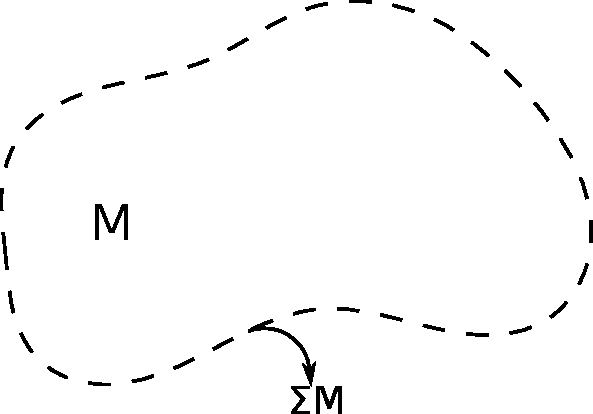
\includegraphics[width=0.25\linewidth]{Chapter 3/Figures/surface.pdf}
            \caption{Representation of the region (manifold $M$) of integration and its surrounding surface$\Sigma M$.}
            \label{fig:surfaceM}
        \end{figure}

        The integral \ref{eq:PointnygDeW} is completely analogous to that in electrodynamics where we integrate the divergence of the Poinying's vector, so we can extend the integration surface $\Sigma M$ to infinity or what is the same \textit{our manifold is asimptotically plane} and the second integral goes to zero, in analogy to electrodynamics we can interpreted the vector $W^{\lambda}$ as a generalyzed four-momentum or heat or losses vector. The variation of the Einstein-Hilbert action then becomes

        \begin{equation}
            \delta S_H[g] = \frac{1}{16\pi}\int_M\left(R_{ab} - \frac{1}{2}Rg_{ab} \right)\delta g^{ab}d^4x,
        \end{equation}

        \begin{equation}
            \frac{\delta S_H[g]}{\delta g^{ab}} = \frac{G_{ab}}{16\pi}.
        \end{equation}

        If we extremalize it we find immediately $G_{ab}=0$ which are the Einstein's equations in the vacuum. 
        
            \subsubsection{Energy-momentum tensor}

        Here we are going to build up the Energy-momentum tensor the hearth of the Einstein's equations and most of the electrodynamics too, to do it we are going to use the Einstein-Hilbert action and a matter action as follows

        \begin{equation}
            S = S_H[g] + S_{matter},
        \end{equation}

        then lets see how changes the variation of the action

        \begin{equation}
            \frac{1}{\sqrt{-g}}\frac{\delta S}{\delta g^{ab}} = \frac{1}{\sqrt{-g}}\left[\frac{\delta S_{H}}{\delta g^{ab}} + \frac{\delta S_m}{\delta g^{ab}} \right],
        \end{equation}

        \begin{equation}
            \frac{1}{\sqrt{-g}}\frac{\delta S}{\delta g^{ab}} = \frac{1}{\sqrt{-g}}\left(\frac{G_{ab}}{16\pi} + \frac{\delta S_m}{\delta g^{ab}} \right)=0,
        \end{equation}

        \begin{equation}
            \frac{1}{\sqrt{-g}}\frac{\delta S_m}{\delta g^{ab}} = -\frac{T_{ab}}{2}\;\rightarrow\; T_{ab}=-\frac{2}{\sqrt{-g}}\frac{\delta S_m}{\delta g^{ab}},
        \end{equation}

        \begin{equation}
            \delta S_m = -\frac{1}{2}\int_M\sqrt{-g}T_{ab}\delta g^{ab}d^4x,
        \end{equation}

        applying variational principles we then arrive to 

        \begin{equation}
            R_{ab}-\frac{1}{2}g_{ab}R = 8\pi T_{ab}.
        \end{equation}

        Thus we've arrived to the Einstein's field equations from variational principles, now we're going to solve this equations but only under the assumption that \textit{the gravitational field is weak but not stationary}. To do it we have to suppose the metric of our manifold is plane with a certain perturbation in a region, so the global metric will be

        \begin{equation}\label{eq:gtensor}
            g_{\alpha\beta} = \eta_{\alpha\beta} + h_{\alpha\beta}\;\;|h_{\alpha\beta}|\ll 1.
        \end{equation}

        Before going further we must prove the tensor \ref{eq:gtensor} is a metric, lets then prove it. The contravariant components of the metric are given by

        \begin{equation}
            g^{\alpha\beta} = \eta^{\alpha\beta} - h^{\alpha\beta}
        \end{equation}

        and given a coordinate chart $\phi = \{x^i\}\;i=0,1,2,3$ and another coordinate chart $\overline{\phi} = \{\overline{x^i}\};i=0,1,2,3$  thus the transformation rule for the metric is

        \begin{equation}
            g_{\overline{\alpha}\overline{\beta}} = \Lambda^{\mu}_{\;\overline{\alpha}}\Lambda^{\nu}_{\;\overline{\beta}}g_{\mu\nu}
        \end{equation}

        where $\Lambda^{\alpha}_{\;\overline{\beta}}$ is a Lorentz Boost then what we see is that the transformation rule is a similarity or translation transformation then

        \begin{equation}
            g_{\overline{\alpha}\overline{\beta}} = \Lambda^{\mu}_{\;\overline{\alpha}}\Lambda^{\nu}_{\;\overline{\beta}}\eta_{\mu\nu} + \Lambda^{\mu}_{\;\overline{\alpha}}\Lambda^{\nu}_{\;\overline{\beta}}h_{\mu\nu} = \eta_{\overline{\alpha} \overline{\beta}} + h_{\overline{\alpha} \overline{\beta}}.
        \end{equation}

        Then $g_{\alpha\beta}$ is effectively a tensor and having a theory invariant under Lorentz transformations implies having at least a special relativistic theory. In the Einstein's equations there is the Ricci's number and tensor, but to calculate them we first have to calculate the Riemann's tensor and the Cristoffel symbols, therefore

        \begin{align*}
            \Gamma^{\mu}_{\;\nu\rho} = \frac{1}{2}g^{\mu\sigma}\left(g_{\sigma\nu,\rho} + g_{\rho\sigma,\nu} - g_{\nu\rho,\sigma} \right)\\
            =\frac{1}{2}\left(\eta^{\mu\sigma} - h^{\mu\sigma} \right)\left[h_{\sigma\nu,\rho} + h_{\rho\sigma,\nu} - h_{\nu\rho,\sigma} \right]\\
            =\frac{1}{2}\eta^{\mu\sigma}\left(h_{\sigma\nu,\rho} + h_{\rho\sigma,\nu} - h_{\nu\rho,\sigma} \right),
        \end{align*}

        \begin{equation}
            R^{\alpha}_{\;\nu\rho\sigma}=\Gamma^{\alpha}_{\;\nu\sigma,\rho}-\Gamma^{\alpha}_{\;\nu\rho,\sigma} + \mathcal{O}(\Gamma^2),
        \end{equation}

        \begin{align*}
            \eta_{\mu\alpha}R^{\alpha}_{\;\nu\rho\sigma}=R_{\mu\nu\rho\sigma}=\frac{\eta_{\mu\alpha}}{2}\left[\eta^{\alpha\beta}\left(h_{\beta\nu,\rho} + h_{\beta\rho,\nu} - h_{\rho\nu,\beta} \right) \right] - \frac{\eta^{\alpha\beta}}{2}\left[ \eta^{\alpha\beta}\left(h_{\beta\nu,\sigma}+h_{\sigma\beta,\nu}-h_{\sigma\nu,\beta} \right)_{,\rho}\right.\\
            \left.-\eta^{\alpha\beta}\left(h_{\beta\nu,\rho} + h_{\rho\beta,\nu} - h_{\rho\nu,\beta} \right)_{,\sigma} \right],
        \end{align*}

        \begin{equation}
            R_{\mu\nu\rho\sigma}=\frac{1}{2}\delta_{\mu}^{\;\beta} \left(h_{\beta\sigma,\nu\rho} + h_{\rho\nu,\beta\sigma} - h_{\sigma\nu,\beta\rho} - h_{\rho'beta,\nu\sigma} \right),
        \end{equation}

        \begin{equation}
            R_{\mu\nu\rho\sigma} = \frac{1}{2}\left(h_{\mu\sigma,\nu\rho} + h_{\rho\nu,\mu\sigma} - h_{\sigma\nu,\mu\rho} - h_{\rho\mu,\nu\sigma} \right)
        \end{equation}


        There the Ricci's curvature tensor is given by

        \begin{equation}
            R_{\mu\nu} = \eta^{\rho}_{\;\alpha} \eta^{\alpha\beta}R_{\alpha\mu\rho\nu} = \frac{1}{2}\left[\partial_{\mu}\partial_{\rho}h^{\rho}_{\:\nu} + \partial^{\rho}\partial_{\nu}h_{\rho\mu} - \partial^{\rho}\partial_{\rho}h_{\nu\mu} - \partial_{\mu}\partial_{\nu}h_{\mu}^{\;\mu} \right]
        \end{equation}
        

        \begin{equation}
            R_{\mu\nu} = \frac{1}{2}\left(\partial_{\rho}\partial_{\mu}h^{\rho}_{\;\nu} + \partial_{\rho}\partial_{\nu}h^{\rho}_{\;\mu} - \partial_{\mu}\partial_{\nu}h - \Box h_{\mu\nu} \right),
        \end{equation}

        where $\Box = \Vec{\nabla}_a\Vec{\nabla}^a$ is the D'Alambertian and in a Minkowski space it corresponds to $\Box = \partial_{\alpha}\partial^{\alpha}$. Well then the Ricci's number is given by

        \begin{equation}
            R = \eta^{\mu\nu}R_{\mu\nu} = \frac{1}{2}\eta^{\mu\nu}\left(\partial_{\rho}\partial_{\mu}h^{\rho}_{\;\nu} + \partial_{\rho}\partial_{\nu}h^{\rho}_{\;\mu} - \partial_{\mu}\partial_{\nu}h - \Box h_{\mu\nu} \right) = \partial_{\rho}\partial_{\mu}h^{\rho\mu}-\Box h.
        \end{equation}

        Now, introducing all of this on the Einstein's field equation we will have the following equation

        \begin{equation}
            \frac{1}{2}\left(\partial_{\rho}\partial_{\mu}h^{\rho}_{\;\nu} + \partial_{\rho}\partial_{\nu}h^{\rho}_{\;\mu} - \partial_{\mu}\partial_{\nu}h - \Box h_{\mu\nu} \right) - \frac{1}{2}\eta_{\mu\nu}\left[\partial_{\rho}\partial_{\sigma}h^{\rho\sigma} - \Box h \right] = 8\pi T_{\mu\nu}.
        \end{equation}

        Before going further there is the needing of introducing a special kind of tensor, called the \textit{inverted trace tensor} which are really useful in the general relativity and in fact, the Einstein's tensor is one of this tensor and we are going to prove it in a moment,  the inverted trace tensor for the perturbation tensor is given by

        \begin{equation}
            \overline{h}_{\mu\nu} = h_{\mu\nu} - \frac{1}{2}h_{\mu\nu}h,
        \end{equation}

        it is easy to see that if we calculated the inverted trace tensor for the Ricci's curvature tensor we get the Einstein's tensor like this:

        \begin{equation}
            \overline{R}_{\alpha\beta}=R_{\alpha\beta}-\frac{1}{2}g_{\alpha\beta}R.
        \end{equation}

        We can then rewrite the perturbation tensor in term of its inverted trace tensor and also its trace as follows

        \begin{equation}
            h_{\mu\nu} = \overline{h}_{\mu\nu} - \frac{1}{2}\eta_{\mu\nu}\overline{h},
        \end{equation}

        \begin{equation}
            \eta^{\mu\nu}\overline{h}_{\mu\nu} = h - 2h = -h = \overline{h}.
        \end{equation}

        Then the Einstein's field equations in terms of the inverted trace tensor becomes

        \begin{align*}
            \partial_{\rho}\partial_{\mu}\left(\overline{h}^{\rho}_{\;\nu} - \frac{1}{2}\delta^{\rho}_{\;\nu}\overline{h} \right) + \partial_{\rho}\partial_{\nu}\left(\overline{h}^{\rho}_{\;\mu} - \frac{1}{2}\delta^{\rho}_{\;\mu}\overline{h} \right) + \partial_{\mu}\partial_{\nu}\overline{h}\\
            -\Box\left(\overline{h}_{\mu\nu} - \frac{1}{2}\eta_{\mu\nu}\overline{h} \right) - \eta_{\mu\nu}\partial_{\rho}\partial_{\sigma}\left(\overline{h}^{\rho\sigma}-\frac{1}{2}\eta^{\rho\sigma}\overline{h} \right) - \eta_{\mu\nu}\Box\overline{h} = 16\pi T_{\mu\nu}
        \end{align*}

        \begin{align*}
            \partial_{\rho}\partial_{\mu}\overline{h}^{\rho}_{\;\nu} - \frac{1}{2}\delta^{\rho}_{\;\nu}\partial_{\rho}\partial_{\mu}\overline{h} + \partial_{\rho}\partial_{\nu}\overline{h}^{\rho}_{\;\mu}-\frac{1}{2}\delta^{\rho}_{\;\mu}\partial_{\rho}\partial_{\nu}\overline{h} + \partial_{\mu}\partial_{\nu}\overline{h} - \Box\overline{h}_{\mu\nu} + \frac{1}{2}\eta_{\mu\nu}\Box\overline{h}\\
            -\eta_{\mu\nu}\partial_{\rho}\partial_{\sigma}\overline{h}^{\rho\sigma} + \frac{1}{2}\eta_{\mu\nu}\eta^{\rho\sigma}\partial_{\rho}\partial_{\sigma}\overline{h}-\eta_{\mu\nu}\Box\overline{h} = 16\pi T_{\mu\nu},\\
            = \partial_{\rho}\partial_{\mu}\eta^{\rho\alpha}\overline{h}_{\alpha\nu}+\partial_{\rho}\partial_{\nu}\eta^{\rho\alpha}\overline{h}_{\alpha\mu} - \frac{1}{2}\delta^{\rho}_{\;\nu}\partial_{\rho}\partial_{\mu}\overline{h} - \frac{1}{2}\delta^{\rho}_{\;\mu}\partial_{\rho}\partial_{\nu}\overline{h} + \partial_{\mu}\partial_{\nu}\overline{h}\\
            -\Box\overline{h}_{\mu\nu} + \frac{1}{2}\eta_{\mu\nu}\Box\overline{h} + \frac{1}{2}\eta_{\mu\nu}\eta^{\rho\sigma}\partial_{\rho}\partial_{\sigma}\overline{h} - \eta_{\mu\nu}\partial_{\rho}\partial_{\sigma}\eta^{\rho\alpha}\eta^{\sigma\beta}\overline{h}_{\alpha\beta}-\eta_{\mu\nu}\Box\overline{h},\\
            =\partial_{\rho}\partial_{\mu}\eta^{\rho\alpha}\overline{h}_{\alpha\nu} + \partial_{\rho}\partial_{\nu}\eta^{\rho\alpha}\overline{h}_{\alpha\mu} - \frac{1}{2}\partial_{\nu}\partial_{\mu}\overline{h} - \frac{1}{2}\partial_{\mu}\partial_{\nu}\overline{h}+\partial_{\mu}\partial_{\nu}\overline{h} - \Box\overline{h}_{\mu\nu}\\
            +\frac{1}{2}\eta_{\mu\nu}\Box\overline{h} + \frac{1}{2}\eta_{\mu\nu}\partial_{\rho}\partial^{\rho}\overline{h} - \eta_{\mu\nu}\eta^{\rho\alpha}\eta^{\sigma\beta}\partial_{\rho}\partial_{\sigma}\overline{h}_{\alpha\beta}- \eta_{\mu\nu}\Box\overline{h},\\
            = \partial_{\rho}\partial_{\mu}\eta^{\rho\alpha}\overline{h}_{\alpha\nu}+\partial_{\rho}\partial_{\nu}\eta^{\rho\alpha}\overline{h}_{\alpha\mu} - \Box\overline{h}_{\mu\nu} - \eta_{\mu\nu}\eta^{\rho\alpha}\eta^{\sigma\beta}\partial_{\rho}\partial_{\sigma}\overline{h}_{\alpha\beta}\\
            = \partial_{\mu}\left[\partial_{\rho}\left(\eta^{\rho\alpha}\overline{h}_{\nu\alpha} \right) \right] + \partial_{\nu}\left[\partial_{\rho}\left(\eta^{\rho\alpha}\overline{h}_{\mu\alpha} \right) \right] - \Box\overline{h}_{\mu\nu} - \eta_{\mu\nu}\eta^{\rho\alpha}\eta^{\sigma\beta}\partial_{\rho}\partial_{\sigma}\overline{h}_{\alpha\beta}\\
            = \partial_{\mu}W_{\nu} + \partial_{\nu}W_{\mu} - \Box\overline{h}_{\mu\nu} - \eta_{\mu\nu}\eta^{\rho\alpha}\eta^{\sigma\beta}\partial_{\rho}\partial_{\sigma}\overline{h}_{\alpha\beta}\\
            = \partial_{\mu}W_{\nu} + \partial_{\nu}W_{\mu} - \Box\overline{h}_{\mu\nu} - \eta_{\mu\nu}\eta^{\rho\alpha}\partial_{\rho}\left[\partial_{\sigma} \left(\eta^{\sigma\beta}\overline{h}_{\alpha\beta} \right) \right],
        \end{align*}

        \begin{equation}
            -\left[\Box\overline{h}_{\mu\nu} - \partial_{\mu}W_{\nu}-\partial_{\nu}W_{\mu} + \eta_{\mu\nu}\eta^{\alpha\beta}\partial_{\alpha}W_{\beta} \right] = 16\pi T_{\mu\nu}
        \end{equation}

Multiplyting both sides by $-1$ and changin $\mu \rightarrow \alpha$ and $\nu \rightarrow \beta$ then we have finally

        \begin{equation}\label{eq:EinsteinEqHbar}
            \Box \overline{h}_{\alpha\beta} - \partial_{\beta}W_{\alpha} - \partial_{\alpha}W_{\beta} + \eta_{\alpha\beta}\eta^{\mu\nu}\partial_{\nu}W_{\mu} = -16\pi T_{\alpha\beta}\;;\;W_{\alpha}= \partial_{\mu}\left(\eta^{\mu\nu}\overline{h}_{\alpha\nu} \right).
        \end{equation}
        The equation \ref{eq:EinsteinEqHbar} is the Eintein's equations and they are really similar to the Maxwell's equations, the terms with $W_{\alpha}$ are like heat o losses fluxes on the borders of the manifold. Our intention now is to convert the equation \ref{eq:EinsteinEqHbar} into a wave equation, but how do we dot? In the same way we do it in electromagnetism! We work with a Gauge theory, a calibration theory, there we use the Lorenz's Gauge, here we hav to find and use this Lorenz's Gauge and later also find out the called \textit{tranverse Gauge}.

